%% =============================================================================
%% An Overview of Inter Coding Tools in AV2
%% Target: IEEE Transactions on Circuits and Systems for Video Technology (TCSVT)
%% Class : IEEEtran (journal mode), bibliography style IEEEtran
%%
%% Figures in figures/*.pdf are vector renderings of the diagrams in
%% ../av2_inter_prediction_overview_final.html (see _work/make_figs.py).
%% Warp and spatial-scan diagrams are drawn below in TikZ with the same palette.
%%
%% Notes for co-authors are typeset in red with \authnote{...}. Set
%% \showauthornotesfalse before submission to hide them.
%% =============================================================================
\documentclass[journal]{IEEEtran}

\usepackage{cite}
\usepackage{amsmath,amssymb,amsfonts}
\usepackage{graphicx}
\usepackage{booktabs}
\usepackage{multirow}
\usepackage{array}
\usepackage{url}
\usepackage[ruled,vlined,linesnumbered]{algorithm2e}
\usepackage{xcolor}
\usepackage{tikz}
\usetikzlibrary{arrows.meta,positioning,calc,patterns}
\usepackage[hidelinks]{hyperref}

% Palette shared with the slide-deck figures.
\definecolor{avblue}{HTML}{0071E3}
\definecolor{avbluesoft}{HTML}{EAF2FC}
\definecolor{avbluemid}{HTML}{7FB5DA}
\definecolor{avorange}{HTML}{FF9500}
\definecolor{avgray}{HTML}{6E6E73}
\definecolor{avgraysoft}{HTML}{EEEEF2}
\definecolor{avred}{HTML}{FF3B30}

\newif\ifshowauthornotes
\showauthornotestrue
\newcommand{\authnote}[1]{\ifshowauthornotes{\color{red}\textbf{[Note: #1]}}\fi}

\newcommand{\code}[1]{\texttt{#1}}
\newcommand{\mvd}{\mathrm{MVD}}

% Let floats share pages with text more freely, so fewer pages are left half
% empty. Float spacing itself is left at the IEEEtran defaults.
\renewcommand{\topfraction}{0.9}
\renewcommand{\dbltopfraction}{0.9}
\renewcommand{\bottomfraction}{0.8}
\renewcommand{\textfraction}{0.07}
\renewcommand{\floatpagefraction}{0.85}
\renewcommand{\dblfloatpagefraction}{0.85}
\setcounter{topnumber}{3}
\setcounter{dbltopnumber}{2}
\setcounter{totalnumber}{4}

\begin{document}

\title{An Overview of Inter Coding Tools in AV2}

\author{Yeqing~Wu$^{*}$,
        Mohammed~Golam~Sarwer$^{*}$,
        Keng-Shih~Lu,
        Jianle~Chen,
        Liang~Zhao,
        Han~Gao,
        Bohan~Li,
        Guoxin~Jin,
        Yunqing~Wang,
        Lin~Zheng,
        Rachel~Barker,
        Jayasingam~Adhuran,
        Jingning~Han,
        Debargha~Mukherjee,
        Hui~Su,
        Yunfei~Zheng,
        Alexis~Tourapis,
        and~Shan~Liu%
\thanks{$^{*}$Y.~Wu and M.~G.~Sarwer are co-first authors.}%
\thanks{Y.~Wu, H.~Gao, G.~Jin, Y.~Zheng, and A.~Tourapis are with Apple Inc., Cupertino, CA, USA.}%
\thanks{M.~G.~Sarwer, K.-S.~Lu, J.~Chen, B.~Li, Y.~Wang, L.~Zheng, J.~Han, D.~Mukherjee, and H.~Su are with Google LLC, Mountain View, CA, USA.}%
\thanks{L.~Zhao, J.~Adhuran, and S.~Liu are with Tencent Media Lab, Palo Alto, CA, USA.}%
\thanks{R.~Barker is with Monocot Ltd., Cambridge, U.K.}%
\thanks{Corresponding authors: Yeqing Wu and Mohammed Golam Sarwer.}}

\markboth{IEEE Transactions on Circuits and Systems for Video Technology}%
{Wu \MakeLowercase{\textit{et al.}}: An Overview of Inter Coding Tools in AV2}

\maketitle

\begin{abstract}
AOMedia Video 2 (AV2) is the next-generation video coding format of the
Alliance for Open Media (AOMedia). It improves coding efficiency over its
predecessor, AOMedia Video 1 (AV1), by
roughly 30\%, and inter prediction is one of the main sources of that gain. This
paper gives a complete, self-contained overview of the inter coding tools in
AV2. We describe what each tool does, why it was designed the way it was, and
what it costs in hardware. The tools fall into five groups. First, a redesigned
reference frame system that stores up to 16 frames and can rank references
implicitly. Second, new prediction tools: Temporal Interpolated Prediction
(TIP), sub-block and optical-flow motion vector (MV) refinement, an extended
family of warped motion modes built around a Warp Reference List, a generalized
wedge mode, an implicit wedge mode for picture boundaries, compound weighted
prediction, and block adaptive weighted prediction. Third, an improved MV
prediction framework that combines a simplified spatial search, trajectory-based
temporal MV prediction with compressed storage, and a reference MV bank. Fourth,
a new MV coding scheme with adaptive and joint MV difference (MVD) coding,
flexible MV resolution, and shell-based MVD entropy coding. Fifth, Backward
Reference Updating (BRU), which lets a decoder update only the changed regions
of a frame in place for low-power, low-latency use cases. Experiments with the
AV2 reference software show the contribution of each tool under random access
and low delay test conditions. For example, TIP alone accounts for 1.40\% of
bit-rate savings in random access, and the warp tools together account for
4.18\% and 5.60\% in random access and low delay, respectively.
\end{abstract}

\begin{IEEEkeywords}
AV2, AV1, AOMedia, video coding, inter prediction, motion compensation,
motion vector prediction, motion vector coding, warped motion, temporal
interpolated prediction.
\end{IEEEkeywords}

%% =============================================================================
\section{Introduction}
\label{sec:intro}
%% =============================================================================

\IEEEPARstart{V}{ideo} makes up most of today's Internet traffic, and the
demand for better compression keeps growing with higher resolutions, higher
frame rates, and new applications such as cloud gaming and screen sharing.
The Alliance for Open Media (AOMedia) was formed in 2015 to develop media
technologies. Its first video format, AOMedia Video 1 (AV1), was finalized in
2018~\cite{av1,av1core} and is now widely deployed. AOMedia Video 2
(AV2)~\cite{av2spec} is the
successor of AV1. It keeps the block-based hybrid coding structure that every
modern video codec uses: each block is predicted from previously decoded pixels
(intra or inter prediction), the prediction error is transformed, quantized,
and entropy coded, and in-loop filters clean up the reconstructed frame. AV2
improves nearly every module of this structure, including a much more flexible
block partitioning, and achieves about 30\% bit-rate savings over AV1 at the
same objective quality.

Inter prediction is the module that removes temporal redundancy, that is, the
similarity between neighboring frames of a video. A block in the current frame
is predicted by copying (and, when needed, interpolating) a block from an
already decoded reference frame, displaced by a motion vector (MV). Only the
difference between the block and its prediction, plus the information needed
to form the prediction, is sent. In natural video the vast majority of frames are inter coded.
Therefore, inter prediction has been a central focus in every generation of
video coding standards, from H.264/Advanced Video Coding (AVC)~\cite{h264} and
H.265/High Efficiency Video Coding (HEVC)~\cite{HEVC} to H.266/Versatile Video
Coding (VVC)~\cite{VVC}, as well as in VP9~\cite{VP9} and AV1~\cite{av1}.

Improving inter coding is a balance of three factors. The first is
\emph{prediction accuracy}: a better prediction leaves a smaller residual.
The second is \emph{side information}: MVs, reference indices, and mode flags
all cost bits, and a tool whose gains are eaten by its own signaling is not
useful. The third is \emph{implementation cost}: memory bandwidth, on-chip
buffer size, and worst-case computation in a hardware decoder. AV2 was
developed with all three in mind. Many of its tools are designed so that the
decoder can \emph{derive} information that would otherwise be signaled (for
example, temporal interpolated prediction (TIP), MV refinement, the implicit
wedge mode, and implicit weight
derivation), and several tools were redesigned specifically to bound memory
use (for example, the spatial MV search, the temporal MV storage, and the
reference MV bank). In the other direction, AV1's overlapped block motion
compensation (OBMC)~\cite{av1obmc}, which is less hardware friendly, was removed
from AV2 in favor of the new tools.

This paper is an overview of all the inter coding tools in AV2. It extends our
two conference papers~\cite{av2inter_icip,av2warp_companion} into a single, unified
description, and adds the background, design rationale, and implementation
details that a short paper cannot include. Our goal is that a reader who knows
the basics of video coding, but not AV1 or AV2, can follow every tool. The
main contributions of the paper are:
\begin{itemize}
  \item a unified description of the AV2 inter coding toolset, organized by
        the stage of the inter coding process it improves (Table~\ref{tab:tool_summary});
  \item for each tool, an explanation of the motivation, the algorithm, the
        signaling, and the measures taken to keep hardware cost low;
  \item a per-tool evaluation with the AV2 reference software under the AOMedia
        common test conditions (CTC), for both random access and low delay
        configurations, including encoder and decoder run times.
\end{itemize}

The rest of the paper is organized as follows. Section~\ref{sec:background}
reviews inter coding in AV1, which is the starting point for AV2.
Section~\ref{sec:refsys} describes the reference frame system.
Section~\ref{sec:pred} presents the inter prediction tools.
Sections~\ref{sec:mvpred} and~\ref{sec:mvcoding} cover MV prediction and MV
coding, respectively. Section~\ref{sec:bru} describes Backward Reference
Updating. Section~\ref{sec:results} reports experimental results, and
Section~\ref{sec:conclusion} concludes the paper.

\begin{table*}[t]
\centering
\caption{Summary of the AV2 inter coding tools covered in this paper, compared with AV1. Section numbers are given in parentheses.}
\label{tab:tool_summary}
\renewcommand{\arraystretch}{1.08}
\setlength{\tabcolsep}{4pt}
\footnotesize
\begin{tabular}{@{}p{2.9cm}p{6.0cm}p{8.6cm}@{}}
\toprule
\textbf{Area} & \textbf{AV1} & \textbf{AV2} \\
\midrule
Reference frames (\ref{sec:refsys})
 & 8 stored frames; 7 references; explicit assignment; 16 compound pairs
 & 16 stored frames; 7 references; explicit or implicit (score-based) ranking; 18 compound pairs \\
New prediction mode (\ref{sec:tip})
 & ---
 & Temporal Interpolated Prediction (TIP): reference mode and direct-output mode \\
MV refinement (\ref{sec:refine})
 & ---
 & Sub-block MV refinement (SMVR); optical-flow MV refinement (OPFL) \\
Warped motion (\ref{sec:warp})
 & Global warp; local warp (least squares, one reference)
 & Warp Reference List; warp-mv, warp-new-mv with delta, warp extend, compound warp causal; short-tap and $4{\times}4$ warp filters \\
Compound masks (\ref{sec:wedge})
 & 16 hand-designed wedge masks per block size
 & Up to 68 parametric wedge masks; implicit wedge mode at picture boundaries \\
Weighted prediction (\ref{sec:weighted})
 & Distance-based weights
 & Compound weighted prediction (signaled weights); block adaptive weighted prediction \\
OBMC
 & Overlapped block motion compensation
 & Removed \\
MV prediction (\ref{sec:mvpred})
 & Spatial search over three rows/columns; linear-projection temporal MV
 & Simplified spatial search, half-size line buffer; trajectory-tracking temporal MV prediction (TMVP) with 16-bit MV storage; reference MV bank \\
MV coding (\ref{sec:mvcoding})
 & 15-bit MV range; frame-level $1/4$ or $1/8$ precision; separable MV difference (MVD) coding
 & 17-bit range; frame- and block-level precision (FMVR); adaptive MVD; joint MVD; shell-based MVD coding \\
Low-power decoding (\ref{sec:bru})
 & ---
 & Backward Reference Updating (BRU) \\
\bottomrule
\end{tabular}
\end{table*}

%% =============================================================================
\section{Background: Inter Coding in AV1}
\label{sec:background}
%% =============================================================================

Since AV2 is built on AV1, we first summarize the parts of AV1 inter coding
that the rest of the paper refers to. A complete description of AV1 can be
found in~\cite{av1,AV1-ATSIP}.

\subsection{Reference Frames}
AV1 keeps up to 8 decoded frames in a decoded picture buffer (DPB), and each inter
frame can choose 7 of them as references, indexed 1 to 7. Indices 1--4 are
meant for frames before the current frame in display order and 5--7 for
frames after it. A block can be predicted from one reference (single
prediction) or from two references (compound prediction). Compound prediction
is either \emph{bi-directional} (one past and one future reference) or
\emph{uni-directional} (both references on the same side). AV1 allows all 12
bi-directional pairs but only 4 uni-directional pairs, for a total of 16
compound pairs.

\subsection{Motion Compensation}
A translational MV in AV1 has $1/8$-pel precision. Sub-pel samples are
produced by separable interpolation filters, and the horizontal and vertical
filters can be chosen independently from three filter types (smooth, regular,
and sharp)~\cite{av1}. Beyond translation, AV1 supports a 6-parameter
\emph{warped} (affine) motion model at the frame level (global motion) and at
the block level (local warp). The local warp model is not signaled; it is
estimated by a least-squares fit to the MVs of neighboring blocks that use the
same reference~\cite{warp-motion}. We review the warp model in more detail in
Section~\ref{sec:warp}.

\subsection{Compound Prediction}
Figure~\ref{fig:compound} shows the idea of compound prediction. The current
block has two MVs, each pointing into a different reference frame, and the two
predictors $P_0$ and $P_1$ are blended:
\begin{equation}
  P = w\,P_0 + (1-w)\,P_1 .
  \label{eq:compound_generic}
\end{equation}
Averaging two predictors reduces noise and handles occlusions and gradual
changes much better than either predictor alone, but the encoder has to send
two MVs. AV1 provides several ways to choose $w$: a constant $w=1/2$
(\code{COMPOUND\_AVERAGE}), a weight that depends on the temporal distances of
the two references, a per-pixel weight based on the difference between $P_0$
and $P_1$, and a \emph{wedge} mode, in which one of 16 predefined masks splits
the block along an oblique line. AV1 also has a combined inter-intra mode and
OBMC, both of which blend a single inter predictor with another signal.

\begin{figure}[t]
  \centering
  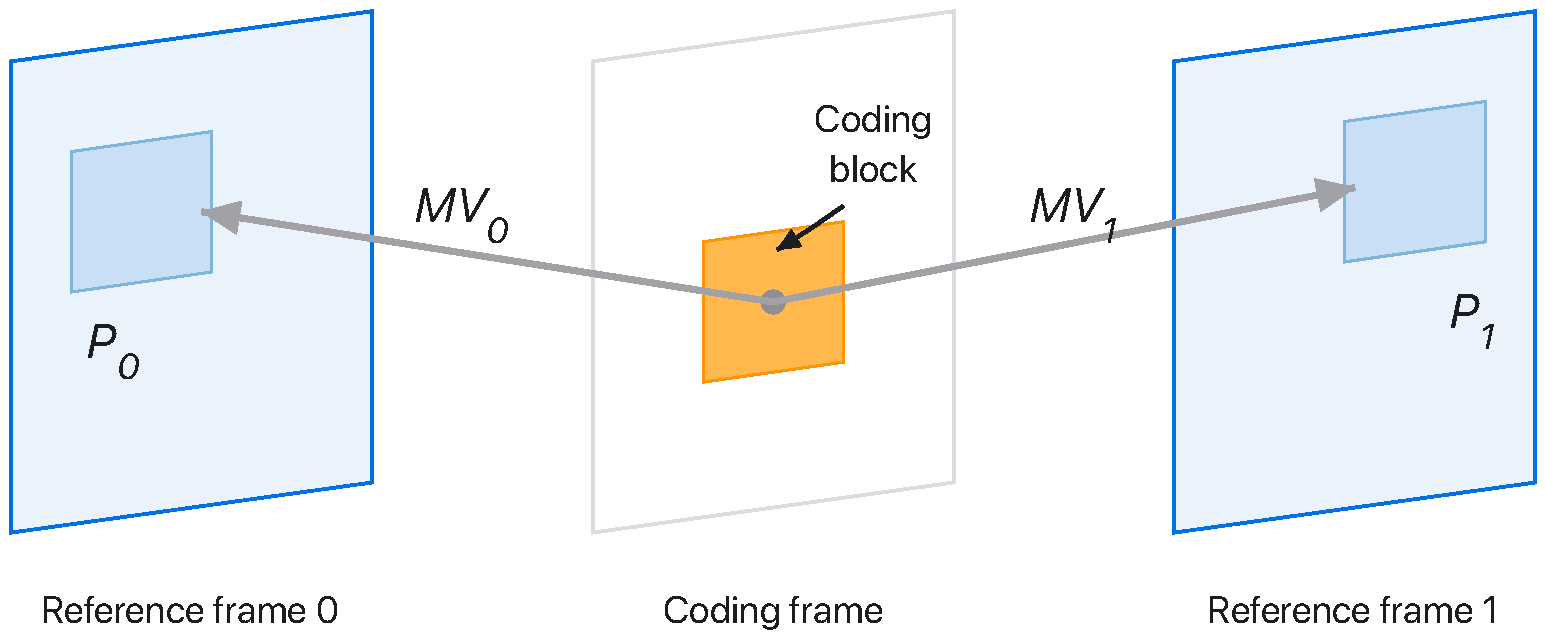
\includegraphics[width=0.80\columnwidth]{figures/compound.pdf}
  \caption{Compound prediction. The coding block is predicted from two
  reference blocks $P_0$ and $P_1$, located by two motion vectors
  $\mathrm{MV}_0$ and $\mathrm{MV}_1$. The prediction is more accurate than
  single prediction, but both MVs must be signaled.}
  \label{fig:compound}
\end{figure}

\subsection{MV Prediction and Coding}
MVs are coded predictively: the encoder sends the difference (MVD) between the
MV and a predictor. AV1 builds a short list of predictor candidates, the
\emph{dynamic reference list} (DRL), from spatial neighbors and from a
temporal motion field, and ranks the candidates by how often they occur
nearby~\cite{MVref}. The temporal candidates come from a motion field that is
built by linearly projecting the MVs stored with the reference frames onto the
current frame. AV1 codes the row and column components of the MVD separately.

%% =============================================================================
\section{Reference Frame System}
\label{sec:refsys}
%% =============================================================================

AV2 doubles the size of the DPB to 16 frames. Each inter frame still uses up
to seven of them as references, but a larger buffer lets the encoder keep
useful frames, such as a long-term background frame or frames from different
layers, for a longer time.

\subsection{Explicit and Implicit Reference Mapping}
AV2 supports two ways to decide which seven frames are used as references.
In \emph{explicit mapping}, as in AV1, the frame header lists which buffer
slot each reference index 1--7 points to. In \emph{implicit mapping}, the
encoder sends nothing. Both the encoder and the decoder compute a score for
every frame in the DPB and pick the seven frames with the lowest scores.
Reference index 1 is the best (lowest-score) frame, index 2 the next, and so
on. The score of a candidate reference frame is
\begin{equation}
  J = J_T + J_R + J_Q + J_L ,
  \label{eq:refscore}
\end{equation}
where each term measures one reason why a frame may be a poor reference:
\begin{itemize}
  \item $J_T$ (temporal distance): frames far away in time are less similar
        to the current frame. If the DPB contains only past frames, $J_T$ is a
        concave, increasing function of the temporal distance; otherwise, it is
        64 times the temporal distance.
  \item $J_R$ (resolution): 32 times the $\log_2$ ratio of the sample counts of
        the current frame and the reference frame. A reference with a
        different resolution must be rescaled before use.
  \item $J_Q$ (quality): the quantization parameter of the reference frame;
        a reference coded with a coarser quantizer is less reliable.
  \item $J_L$ (layer): the absolute difference between the layer identifiers of the
        current and reference frames.
\end{itemize}
Implicit mapping saves the header bits of explicit mapping, and, more
importantly, it gives every inter frame a consistent ordering of its
references: low indices always mean ``more useful''. AV2 exploits this
ordering in compound prediction.

\subsection{Compound Reference Pairs}
Single prediction may use any of the seven references. For compound
prediction, AV2 allows only the pairs $(a,b)$ with $1\le a\le 3$ and
$a\le b\le 7$, i.e., every allowed pair contains at least one of the three
best-ranked references. For example, $(1,5)$ is allowed but $(4,7)$ is not.
This gives $7+6+5=18$ pairs. Note that pairs $(1,1)$, $(2,2)$, and $(3,3)$
are allowed, i.e., compound prediction with two different MVs into the
\emph{same} reference frame. Restricting the
pairs keeps the signaling of the reference pair cheap.

%% =============================================================================
\section{Inter Prediction Tools}
\label{sec:pred}
%% =============================================================================

\subsection{Temporal Interpolated Prediction (TIP)}
\label{sec:tip}

\subsubsection{Motivation}
Compound prediction gives an accurate prediction, but it costs two MVs.
Many blocks, however, move in a way that is already described by the motion
of the reference frames: if an object moves steadily from frame $F_{i-1}$ to
frame $F_{i+1}$, its position in the frame in between, $F_i$, can be
predicted without sending any new motion. TIP~\cite{tip,tip_ld,tip_opfl,tip_weights}
uses this idea. It builds an interpolated frame, the \emph{TIP frame}, at the
time instant of the current frame, from MVs that the decoder already has. The
TIP frame combines two references, so it has the accuracy of compound
prediction, while a block that uses it needs at most one MV.

\begin{figure*}[t]
  \centering
  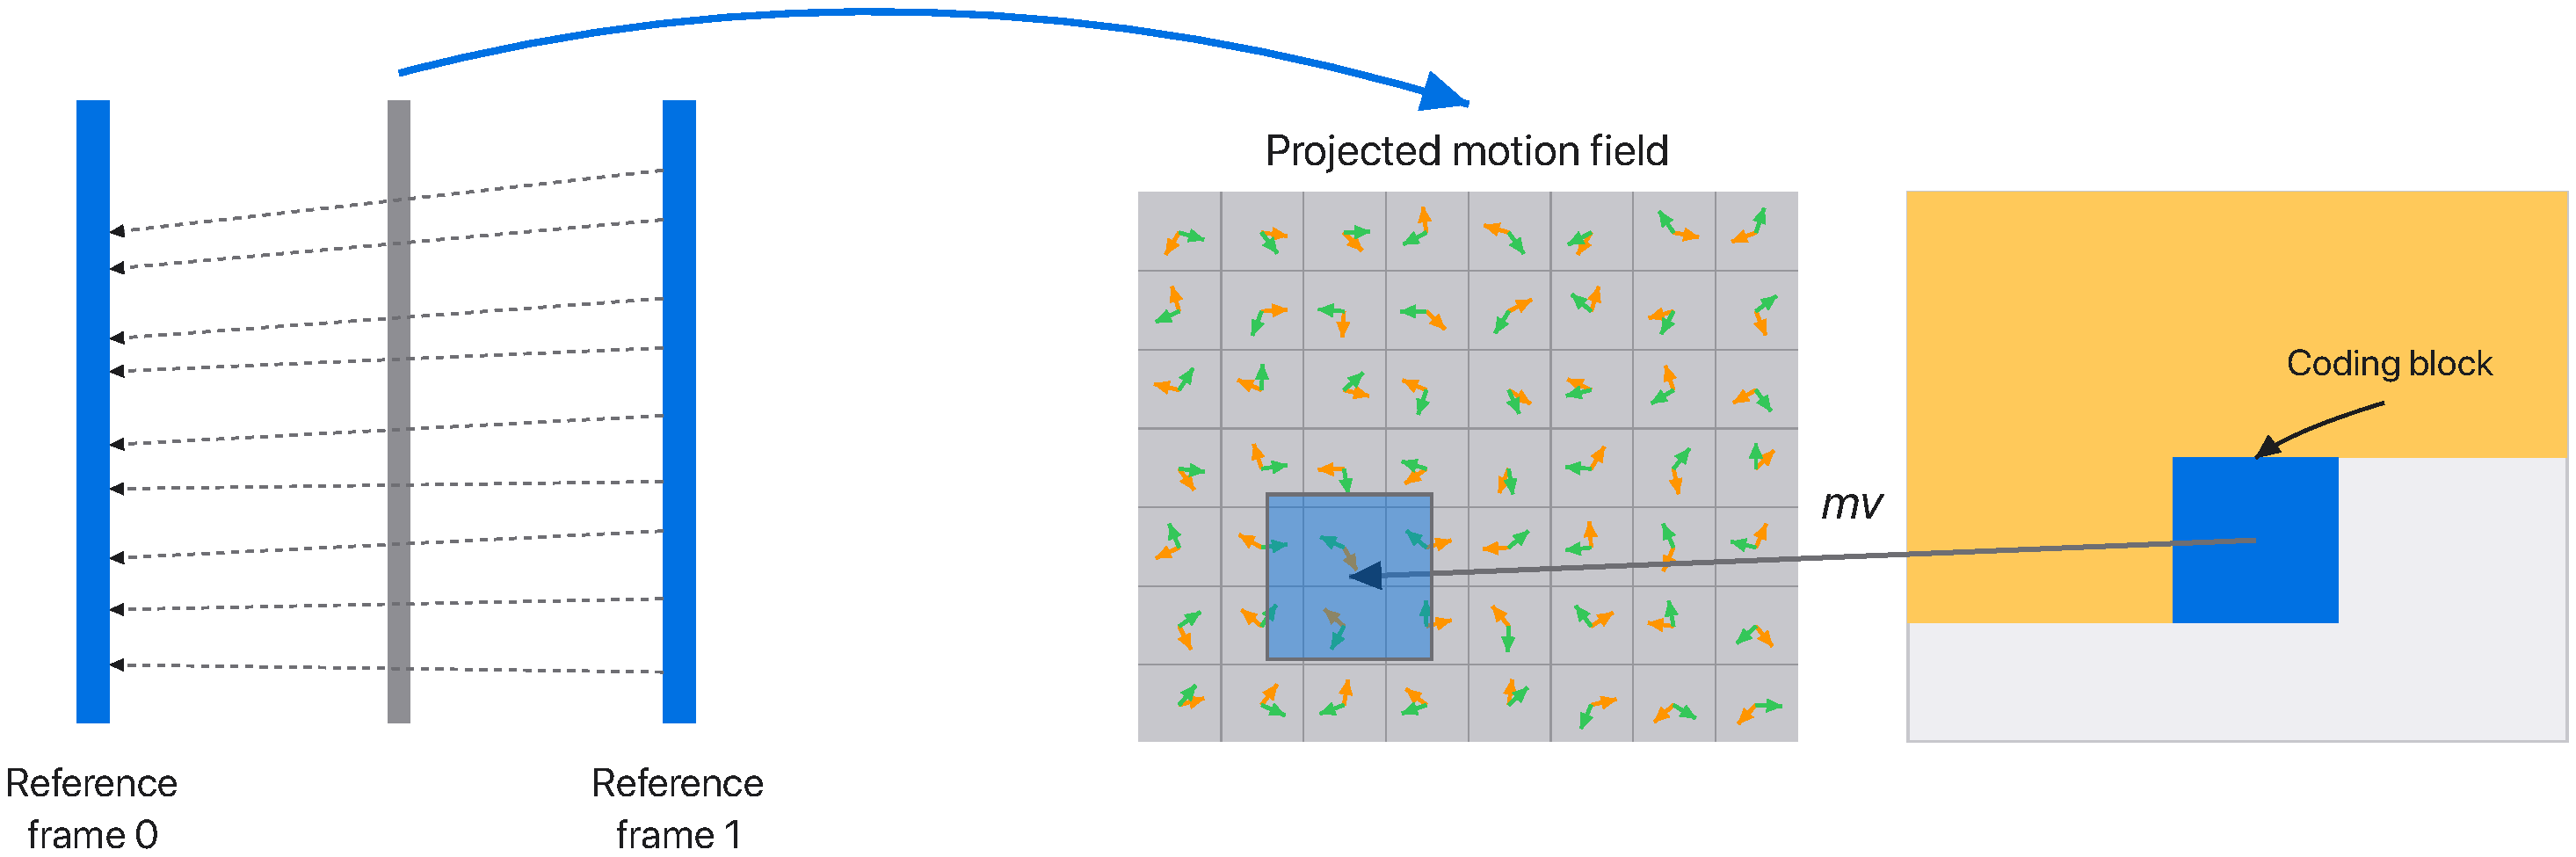
\includegraphics[width=0.80\textwidth]{figures/tip_concept.pdf}
  \caption{Temporal Interpolated Prediction. Left: MVs that are already
  stored with the reference frames (dashed arrows) are projected onto the
  time instant of the current frame. Middle: this gives a motion field for the
  current frame, with one MV towards each of the two references (orange and
  green arrows) for each $8{\times}8$ block. Right: a coding block in the
  current frame (blue) references the TIP frame with a single MV $mv$; the
  orange area is already coded.}
  \label{fig:tip_concept}
\end{figure*}

\subsubsection{Building the TIP Frame}
TIP does not perform any new motion estimation. It reuses the projected
motion field that is built for temporal MV prediction (TMVP,
Section~\ref{sec:tmvp}). As shown in Fig.~\ref{fig:tip_concept}, MVs stored
with the reference frames are projected onto the current frame, which gives,
for each $8{\times}8$ block of the current frame, an estimate of where that
block came from in the two references used by TIP. Only one projected MV
($mfmv$) is stored per block; the two MVs towards the two TIP references,
$mfmv_0$ and $mfmv_1$, are derived from it on the fly by scaling with the
temporal distances.

The two references used to build the TIP frame are chosen as follows. If the
current frame has references both in the past and in the future, TIP uses the
closest past reference and the closest future reference (interpolation). If
all references are on the same side, as in low delay coding, TIP uses the two
closest references in that direction (extrapolation). The same framework also
works with a single reference.

Importantly, the TIP frame is never built as a whole frame in memory. The AV2
decoder produces TIP samples block by block, on the fly, as part of the normal
block-based prediction pipeline, in a single pass. This keeps TIP compatible
with hardware decoders that process one superblock at a time.

\subsubsection{Two TIP Modes}
\begin{itemize}
  \item \emph{TIP reference mode.} The TIP frame is used as an additional
        reference frame. A block can choose the TIP frame as its reference and
        send one MV (which may be zero) relative to it. Since each TIP sample
        is already the blend of two references, such a block gets
        bi-prediction-like quality for close to the cost of a single
        prediction.
  \item \emph{TIP direct output mode.} The TIP frame is used directly as the
        reconstructed current frame. Apart from a frame-level MV offset,
        nothing is coded for the frame: no block modes, no residual. This is
        very efficient at low bit rates and also reduces both encoder and
        decoder work for that frame.
\end{itemize}

\begin{figure*}[t]
  \centering
  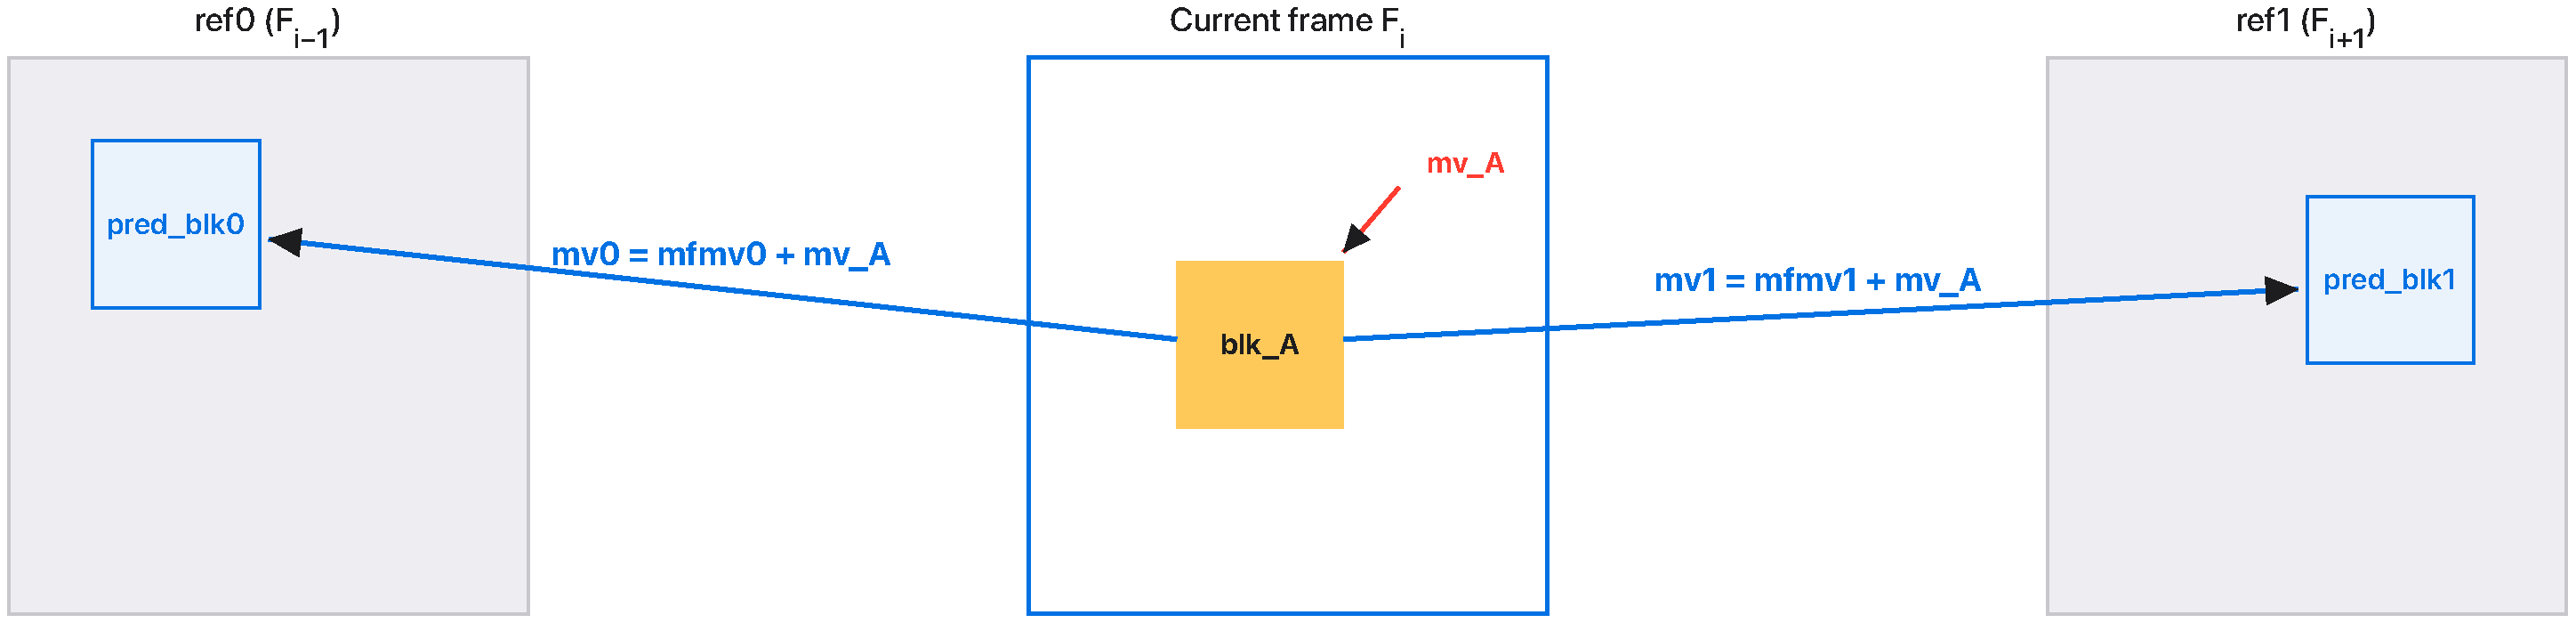
\includegraphics[width=0.80\textwidth]{figures/tip_block.pdf}
  \caption{Block-level TIP reconstruction. For block $blk\_A$, only $mv\_A$
  is parsed. The projected MVs $mfmv0$ and $mfmv1$ come from the TMVP motion
  field at the collocated position. The two predictors are formed with
  $mv0 = mfmv0 + mv\_A$ and $mv1 = mfmv1 + mv\_A$ and then averaged.}
  \label{fig:tip_block}
\end{figure*}

\subsubsection{Block-Level Reconstruction}
Fig.~\ref{fig:tip_block} shows how a block $blk\_A$ is reconstructed with
TIP. The decoder (1) identifies, at the frame level, the two references
$ref0$ and $ref1$ used by TIP; (2) parses $mv\_A$, which is the block MV in
TIP reference mode and the frame-level offset MV in TIP direct output mode;
(3) reads $mfmv0$ and $mfmv1$ from the TMVP motion field at the position
collocated with $blk\_A$; and (4) forms two predictors with
$mv0 = mfmv0 + mv\_A$ on $ref0$ and $mv1 = mfmv1 + mv\_A$ on $ref1$, and
combines them.
Because the projected motion field is defined on an $8{\times}8$ grid, a large
TIP block is in effect predicted with a separate pair of MVs for every
$8{\times}8$ sub-block, which tracks motion variations inside the block at no
signaling cost.

\subsubsection{Weighted TIP and Refinement}
By default the two TIP predictors are averaged. When MV refinement is not
used, the encoder can instead choose one of eight weights at the frame level,
\begin{equation}
  P(x,y) = \frac{W\,P_0(x,y) + (16-W)\,P_1(x,y)}{16},
  \label{eq:tip_weight}
\end{equation}
with $W\in\{8, 12, 16, 18, 20, 4, 6, -4\}$, where $P_0$ comes from the
temporally closer reference. $W=16$ turns TIP into single prediction from the
closer reference, and weights outside $[0,16]$ ($W=18, 20, -4$) extrapolate
from the two predictors. The encoder applies the same weight to
luma and chroma, picks the weight that minimizes the sum of squared errors
between the TIP frame and the source, and signals its index.

The projected motion field is only an estimate. To improve it, the
decoder-side refinements of Section~\ref{sec:refine}, SMVR and OPFL, can be
applied on top of TIP. These refinements assume equal weighting, so when they
are enabled, $W=8$ is used and no weight index is signaled.

\subsection{Decoder-Side MV Refinement}
\label{sec:refine}

In bi-directional compound prediction, the two predictors $P_0$ and $P_1$
should look the same if the MVs are correct: both are supposed to show the
current block, one seen from the past and one from the future. AV2 uses this
property to improve the MVs at the decoder, without any extra signaling. Two
complementary tools are used: a small block-matching search (SMVR) that
corrects integer-pel errors, and an optical-flow solution (OPFL) that
corrects small sub-pel errors.

\subsubsection{Sub-Block MV Refinement (SMVR)}
\label{sec:smvr}
SMVR~\cite{av2smvr} applies to compound blocks whose two references are on
opposite sides of the current frame at equal temporal distances. As shown in
Fig.~\ref{fig:smvr}, a block larger than $16{\times}16$ is split into
$16{\times}16$ sub-blocks; a smaller block is treated as a single sub-block.
For each sub-block, the decoder tests offsets $\Delta mv$ in a $5{\times}5$
integer-pel window around the initial MVs. The offset is applied in
\emph{mirrored} form,
\begin{equation}
  P_0 = \mathrm{ref0}(\mathrm{MV}_0 + \Delta mv),\quad
  P_1 = \mathrm{ref1}(\mathrm{MV}_1 - \Delta mv),
  \label{eq:smvr}
\end{equation}
because, for equal temporal distances, a motion error in one direction shows
up with the opposite sign in the other direction. The decoder chooses the
offset that minimizes the sum of absolute differences (SAD) between $P_0$ and
$P_1$:
\begin{equation}
  \Delta mv^{*} = \arg\min_{\Delta mv}\ \mathrm{SAD}\big(P_0, P_1\big).
\end{equation}
The refined MVs are $\mathrm{MV}_0 + \Delta mv^{*}$ and
$\mathrm{MV}_1 - \Delta mv^{*}$. Note that the search does not need the source
video, so the decoder can repeat it exactly.

\begin{figure*}[t]
  \centering
  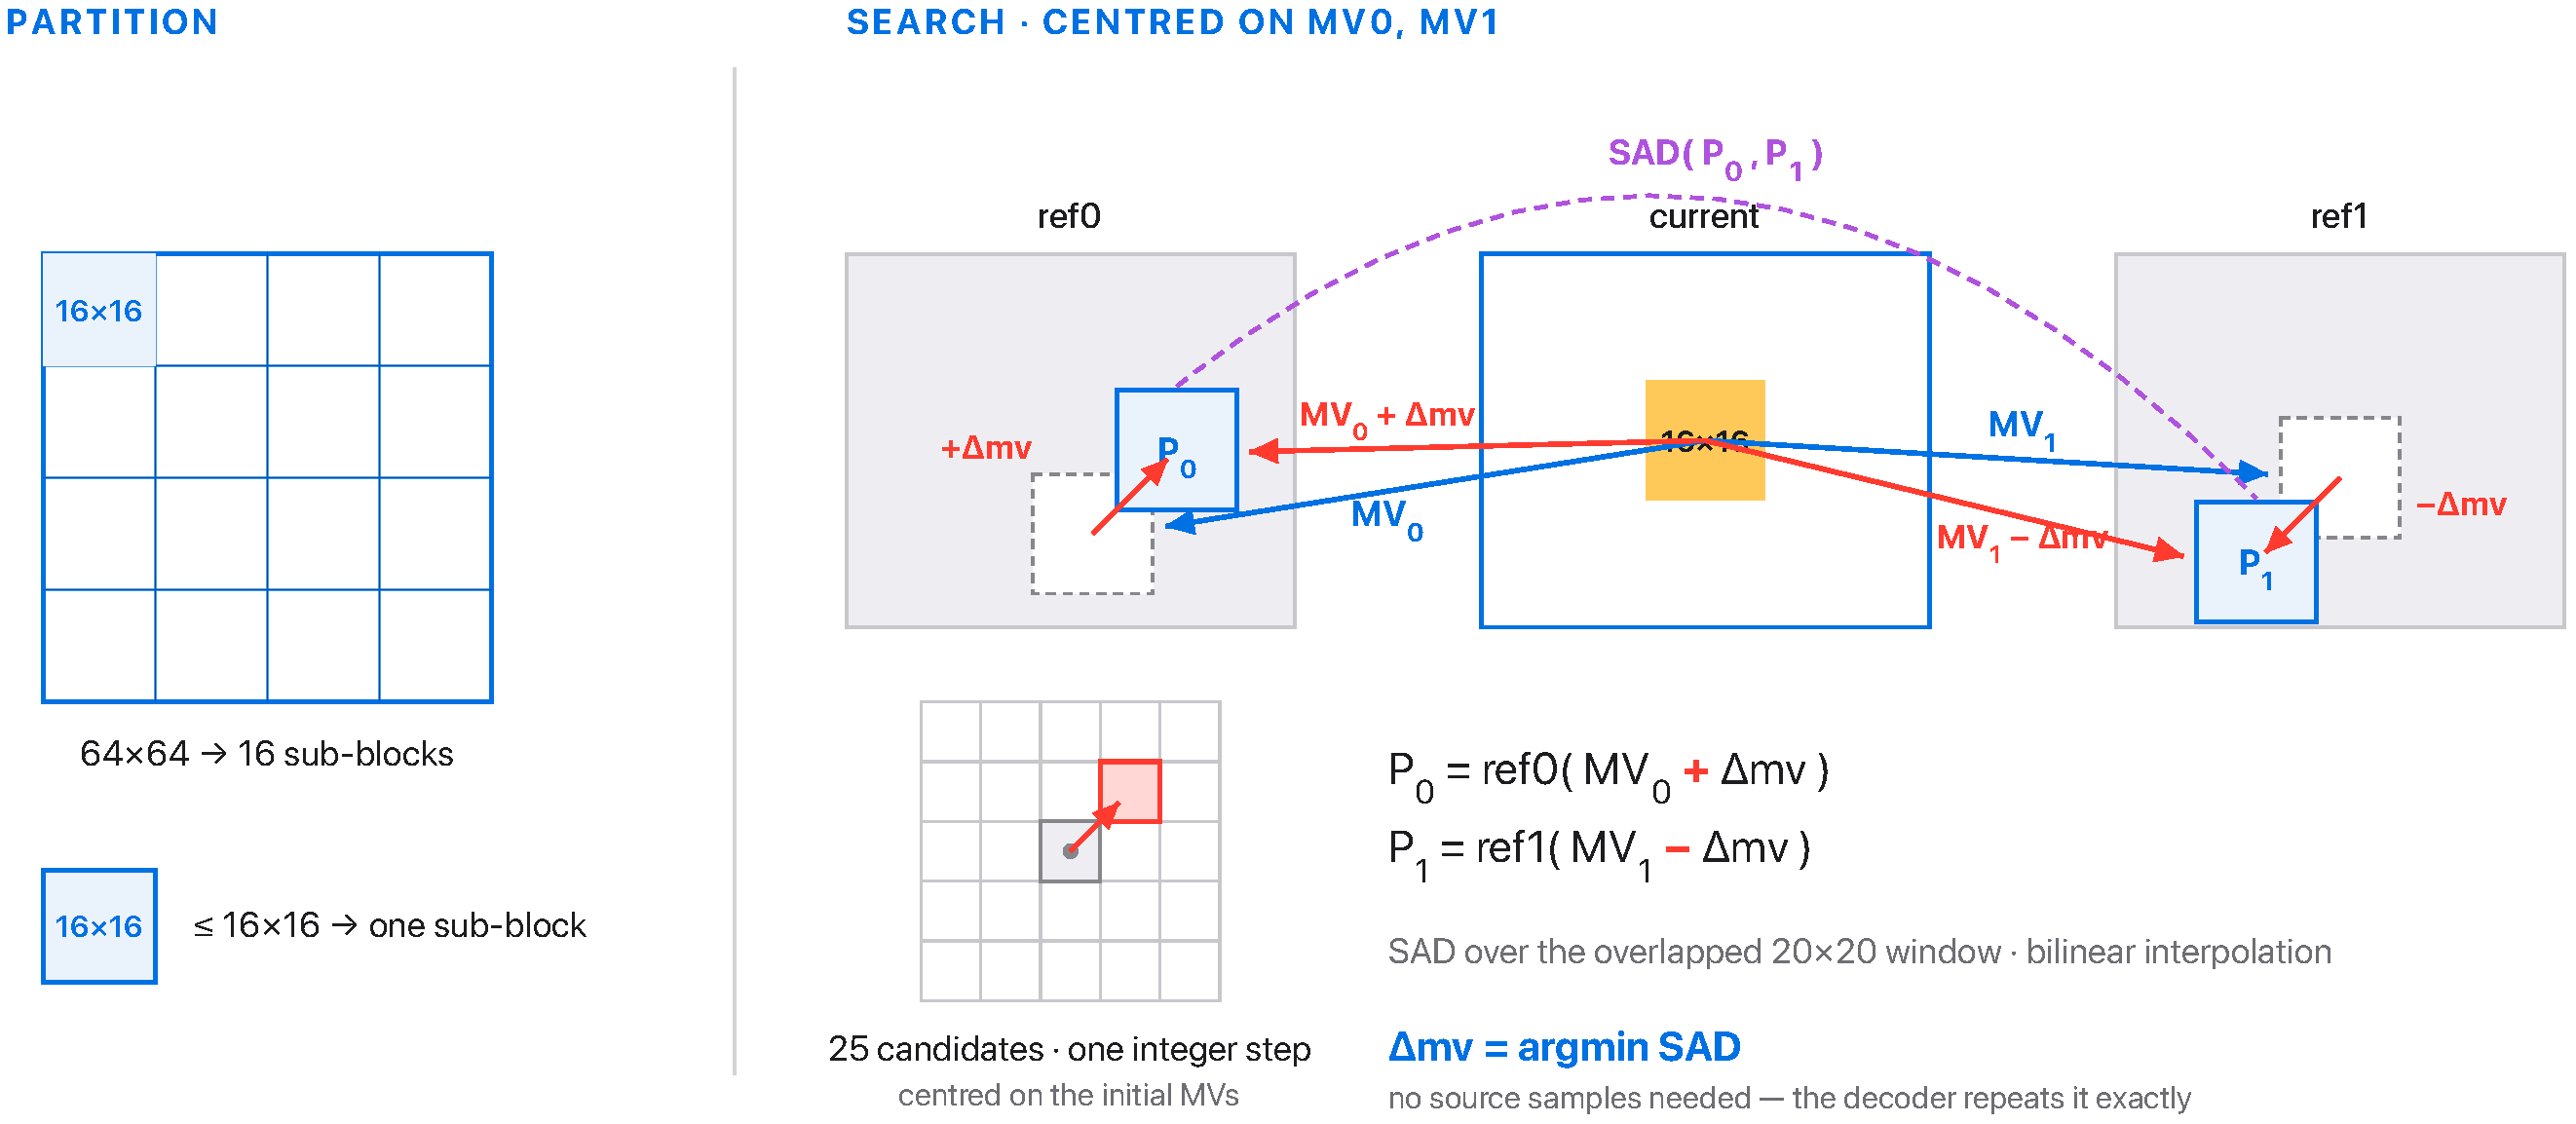
\includegraphics[width=0.72\textwidth]{figures/smvr.pdf}
  \caption{Sub-block MV refinement (SMVR). Left: a $64{\times}64$ block is split
  into sixteen $16{\times}16$ sub-blocks; a block of $16{\times}16$ or less is
  one sub-block. Right: for each sub-block, 25 integer offsets $\Delta mv$
  around the initial MVs are tested. $P_0$ moves by $+\Delta mv$ and $P_1$ by
  $-\Delta mv$, and the offset with the smallest SAD between $P_0$ and $P_1$
  is kept.}
  \label{fig:smvr}
\end{figure*}

Several details keep SMVR cheap. The SAD is computed on predictors made with a
bilinear filter instead of the full interpolation filter. To make the result
robust, the SAD of a $16{\times}16$ sub-block is evaluated on a
$20{\times}20$ window that overlaps the neighboring sub-blocks by 2 samples on
each side. SMVR is allowed only for blocks larger than $8{\times}8$. It is
controlled by a block-level flag, \code{refinemv\_flag}. For
\code{NEAR\_NEARMV} (both MVs taken from the predictor list without an MVD)
and for TIP blocks, the flag is not sent and is inferred to be 1; for other
eligible modes it is signaled.

A key hardware issue is the reference fetch. A hardware decoder loads the
reference samples needed by the \emph{initial} MVs from external memory before
motion compensation. A refined MV may need samples outside this area. To
avoid a second fetch, AV2 fills any sample outside the fetched area by
padding. This keeps the memory bandwidth of
SMVR the same as that of regular compound prediction.

\subsubsection{Optical-Flow MV Refinement (OPFL)}
\label{sec:opfl}
OPFL estimates a small, sub-pel motion correction in closed form. It is based
on bi-directional optical flow (BDOF)~\cite{alshin2010bi-directional}, as used
in VVC~\cite{vvc_subblock}, generalized so that it also works when the two
temporal distances are not equal~\cite{lu2021generalized}.

\begin{figure*}[t]
  \centering
  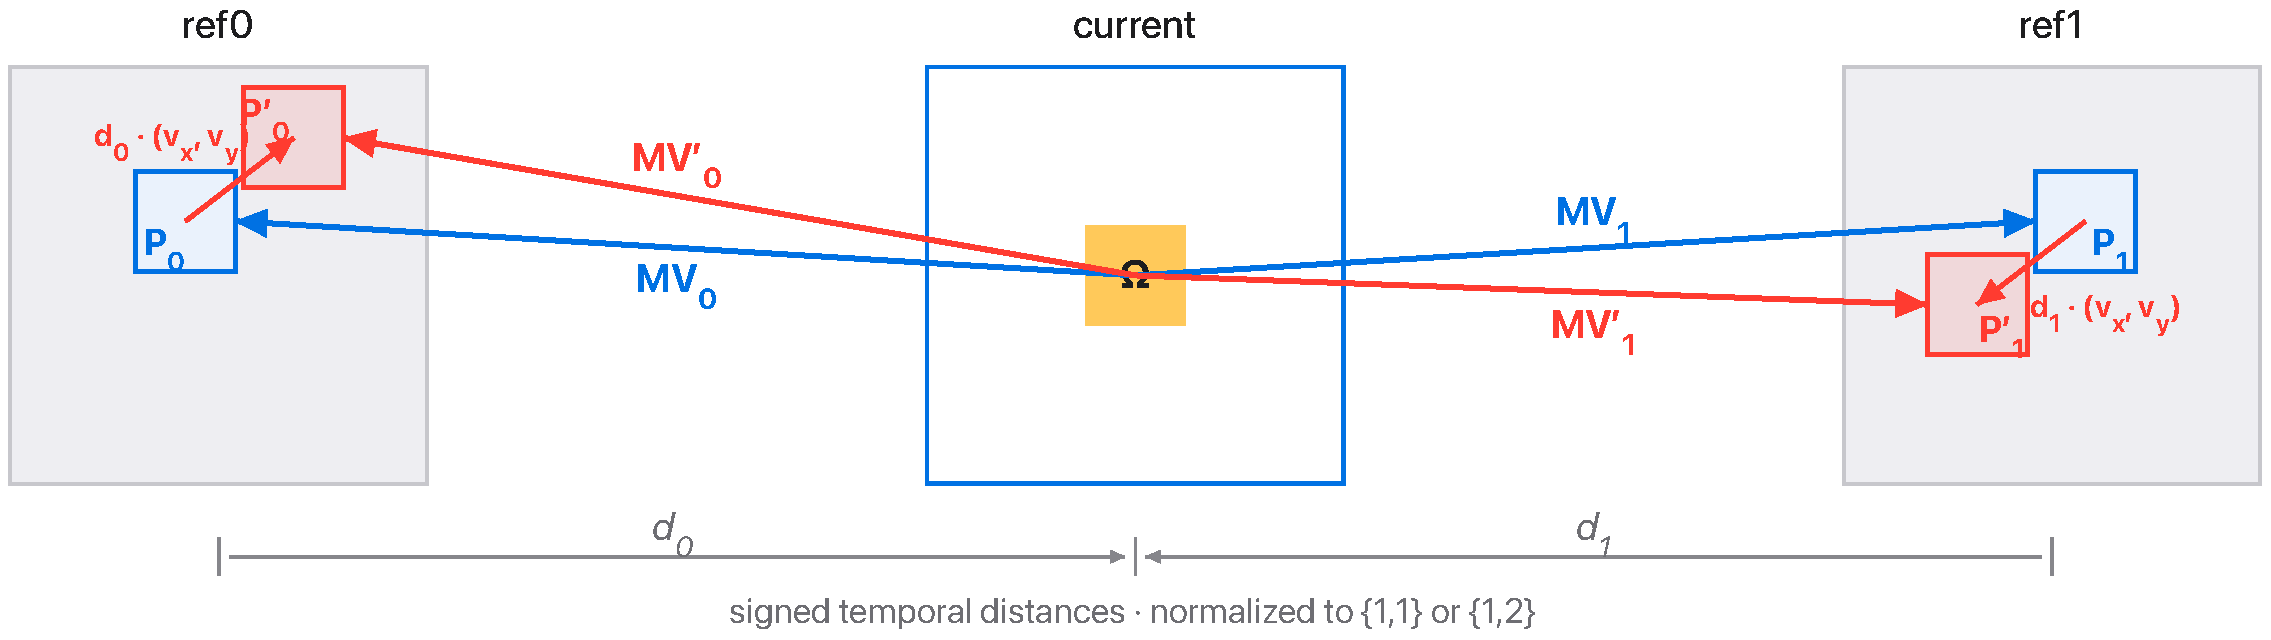
\includegraphics[width=0.76\textwidth]{figures/opfl.pdf}
  \caption{Optical-flow MV refinement (OPFL). For each sub-block $\Omega$, a
  displacement $(v_x, v_y)$ is solved in closed form from the two initial
  predictors $P_0$ and $P_1$. Each MV is then corrected in proportion to its
  signed temporal distance, $\mathrm{MV}_i' = \mathrm{MV}_i + d_i\,(v_x,v_y)$.
  Nothing is signaled.}
  \label{fig:opfl}
\end{figure*}

The idea is illustrated in Fig.~\ref{fig:opfl}. Let $d_0$ and $d_1$ be the
signed temporal distances from the current frame to the two references.
Suppose that, inside a small sub-block $\Omega$, the true motion differs from
the initial MVs by a constant velocity $(v_x, v_y)$ per unit of time. Then the
reference block in $\mathrm{ref}_i$ should be shifted by $d_i(v_x,v_y)$. If
the shift is small, a first-order Taylor expansion shows that the two shifted
predictors agree when
\begin{equation}
  G_t(x,y) + v_x G_x(x,y) + v_y G_y(x,y) \approx 0, \quad (x,y)\in\Omega,
  \label{eq:of_constraint}
\end{equation}
where $G_t = P_0 - P_1$ is the temporal difference and $G_x$ and $G_y$ are the
horizontal and vertical gradients of the distance-weighted difference
$T = d_0P_0 - d_1P_1$. Equation~\eqref{eq:of_constraint} gives one equation
per sample but only two unknowns, so OPFL solves it in the least-squares
sense, minimizing $\sum_{\Omega}\big(G_t + v_xG_x + v_yG_y\big)^2$. With
$S_{ab} = \sum_{(x,y)\in\Omega} G_a G_b$, the solution is
\begin{align}
  v_x &= \frac{S_{ty}S_{xy} - S_{tx}S_{yy}}{S_{xx}S_{yy} - S_{xy}^2}, \label{eq:vx}\\
  v_y &= \frac{S_{tx}S_{xy} - S_{ty}S_{xx}}{S_{xx}S_{yy} - S_{xy}^2}. \label{eq:vy}
\end{align}
The refined MVs are $\mathrm{MV}_i' = \mathrm{MV}_i + d_i(v_x, v_y)$, and the
sub-block is predicted again with the refined MVs and averaged.

In summary, OPFL proceeds in five steps: (i) form $P_0$ and $P_1$ by motion
compensation; (ii) compute $T$ and $G_t$; (iii) compute $G_x$ and $G_y$ from
$T$; (iv) solve~\eqref{eq:vx}--\eqref{eq:vy} for each sub-block; and (v)
apply the refined MVs and average. The following restrictions keep OPFL
simple:
\begin{itemize}
  \item it is used only with two references on opposite sides and with simple
        averaging (not with wedge or weighted compound prediction);
  \item the derivation uses luma only, and the chroma blocks reuse the
        luma result;
  \item $|d_0|$ and $|d_1|$ are normalized to $\{1,1\}$ if they are equal and
        to $\{1,2\}$ otherwise, so that the scaling needs only shifts;
  \item the sub-block size is $8{\times}8$ when OPFL is used with TIP or after
        SMVR; otherwise it is $4{\times}4$ for $8{\times}8$ blocks and
        $8{\times}8$ for larger blocks.
\end{itemize}

\subsubsection{How SMVR and OPFL Work Together}
SMVR and OPFL target different error sizes. SMVR is a search, so it can fix
errors of one or two pels but has integer resolution. OPFL is a linearization,
so it is precise for small errors but breaks down for large ones. When both
apply to a block, SMVR runs first, and OPFL then refines the result on
$8{\times}8$ sub-blocks. Both tools can also refine TIP predictions
(Section~\ref{sec:tip}).

\subsection{Warped Motion Prediction}
\label{sec:warp}

Translational motion cannot describe zoom, rotation, or perspective change.
Affine (warped) motion models address this and are part of VVC~\cite{affine_4param,vvc_subblock}
and AV1~\cite{warp-motion}. AV2 greatly extends the warp tools of
AV1~\cite{av2warp_companion,warp_beyond_av1}. We first review the warp model
of AV1 and then describe the new AV2 tools.

\subsubsection{Warp Model in AV1}
A warp model maps a pixel at $(x,y)$ in the current frame to a position
$(x',y')$ in the reference frame:
\begin{equation}
  \begin{bmatrix} x' \\ y' \end{bmatrix} =
  \begin{bmatrix} h_{11} & h_{12} & h_{13} \\ h_{21} & h_{22} & h_{23} \end{bmatrix}
  \begin{bmatrix} x \\ y \\ 1 \end{bmatrix}.
  \label{eq:warp_model}
\end{equation}
We call $(h_{13},h_{23})$ the \emph{translational} parameters (they play the
role of a regular MV) and $(h_{11},h_{12},h_{21},h_{22})$ the
\emph{non-translational} parameters (they describe scaling, rotation, and
shear). AV1 has a global warp model per reference frame and a local warp mode
at the block level. In local warp, only the translational part is signaled;
the other four parameters are estimated by a least-squares fit to the MVs of
neighboring blocks that use the same reference~\cite{warp-motion}.

To make warped prediction affordable, AV1 splits the $2{\times}2$ part of the
model into two shears,
\begin{equation}
  \begin{bmatrix} h_{11} & h_{12} \\ h_{21} & h_{22} \end{bmatrix} =
  \begin{bmatrix} 1 & 0 \\ \gamma & 1+\delta \end{bmatrix}
  \begin{bmatrix} 1+\alpha & \beta \\ 0 & 1 \end{bmatrix},
  \label{eq:shear}
\end{equation}
so that an $8{\times}8$ block can be predicted by a horizontal filter pass and
a vertical filter pass, much like a translational block, except that the
filter phase changes from pixel to pixel. To bound the reference area of an
$8{\times}8$ block to $15{\times}15$ samples with 8-tap filters, AV1 requires
\begin{equation}
  4|\alpha| + 7|\beta| < 1 \quad\text{and}\quad 4|\gamma| + 4|\delta| < 1 .
  \label{eq:warp_valid}
\end{equation}
This is a strong limit: it rules out the large zooms and rotations where warp
prediction would help the most.

The AV1 design has two other weaknesses. The least-squares model depends
entirely on the neighbors and cannot be corrected when it is wrong. And
signaling a full model explicitly, the obvious alternative, is expensive. AV2
addresses these weaknesses with a list of candidate models, cheap ways to
signal corrections, a mode that extends a neighbor's model, compound warp, and
new prediction filters for large models.

\subsubsection{Warp Reference List (WRL)}
\label{sec:wrl}
Much like the DRL provides MV predictors, the WRL provides candidate warp
models, so that a block can pick a model with a short index instead of
signaling six parameters. The WRL has four entries and is built from
previously decoded information in four steps.

\begin{figure}[t]
  \centering
  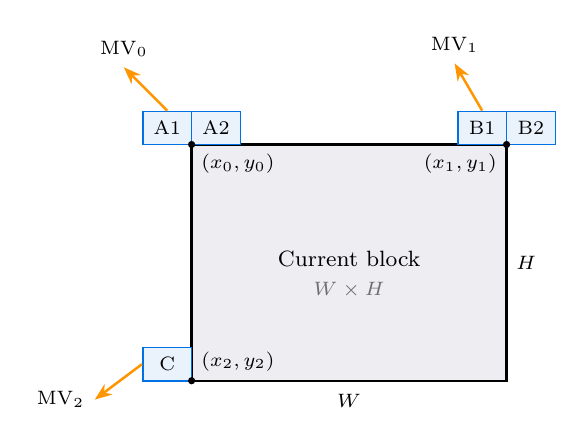
\begin{tikzpicture}[x=1cm,y=1cm,
      nb/.style={draw=avblue, fill=avbluesoft, line width=0.6pt, minimum width=0.62cm, minimum height=0.42cm, font=\scriptsize, inner sep=0pt},
      mv/.style={-{Stealth[length=2.2mm]}, avorange, line width=0.9pt}]
    % current block
    \draw[line width=0.8pt, fill=avgraysoft] (0,0) rectangle (4,3);
    \node[font=\footnotesize] at (2,1.55) {Current block};
    \node[font=\scriptsize, avgray] at (2,1.15) {$W \times H$};
    % corner neighbors
    \node[nb] (A1) at (-0.31,3.21) {A1};
    \node[nb] (A2) at ( 0.31,3.21) {A2};
    \node[nb] (B1) at ( 3.69,3.21) {B1};
    \node[nb] (B2) at ( 4.31,3.21) {B2};
    \node[nb] (C)  at (-0.31,0.21) {C};
    % corner points
    \fill (0,3) circle (1.3pt) node[below right, font=\scriptsize] {$(x_0,y_0)$};
    \fill (4,3) circle (1.3pt) node[below left,  font=\scriptsize] {$(x_1,y_1)$};
    \fill (0,0) circle (1.3pt) node[above right, font=\scriptsize] {$(x_2,y_2)$};
    % MVs
    \draw[mv] (A1.north) -- ++(-0.55,0.55) node[above, font=\scriptsize, black] {$\mathrm{MV}_0$};
    \draw[mv] (B1.north) -- ++(-0.35,0.6) node[above, font=\scriptsize, black] {$\mathrm{MV}_1$};
    \draw[mv] (C.west) -- ++(-0.6,-0.45) node[left, font=\scriptsize, black] {$\mathrm{MV}_2$};
    \node[font=\scriptsize] at (2,-0.25) {$W$};
    \node[font=\scriptsize] at (4.25,1.5) {$H$};
  \end{tikzpicture}
  \caption{Warp model from three corners. The MVs of the neighbors at the
  top-left (A1 or A2), top-right (B1 or B2), and bottom-left (C) corners of
  the current block move its three corners; the warp model that produces
  these three motions is computed with~\eqref{eq:corner_h11}--\eqref{eq:corner_h23}.}
  \label{fig:warp_corner}
\end{figure}

\emph{Step 1: model from three corners.} As shown in
Fig.~\ref{fig:warp_corner}, the decoder looks at neighbors at the top-left,
top-right, and bottom-left corners of the current block, first the set
(A1, B1, C) and, if that set is not usable, the set (A2, B2, C). A set is
usable if all three neighbors are inter coded and use the same reference as
the current block. Their MVs, $\mathrm{MV}_0$, $\mathrm{MV}_1$, and
$\mathrm{MV}_2$, move the corners $(x_0,y_0)$, $(x_1,y_1)$, and $(x_2,y_2)$ of
the block to $(x'_k, y'_k) = (x_k,y_k) + \mathrm{MV}_k$. Three point pairs
determine an affine model exactly. With block width $W$ and height $H$
(powers of two), the solution needs only subtractions and shifts:
\begin{align}
  h_{11} &= (x'_1 - x'_0) \gg \log_2 W, &
  h_{12} &= (x'_2 - x'_0) \gg \log_2 H, \label{eq:corner_h11}\\
  h_{21} &= (y'_1 - y'_0) \gg \log_2 W, &
  h_{22} &= (y'_2 - y'_0) \gg \log_2 H, \\
  h_{13} &= x'_0 - h_{11}x_0 - h_{12}y_0, &
  h_{23} &= y'_0 - h_{21}x_0 - h_{22}y_0. \label{eq:corner_h23}
\end{align}
If a model is found, it becomes the first WRL entry.

\emph{Step 2: spatial neighbors.} The decoder visits the spatial neighbors
in the same order used to build the DRL (Fig.~\ref{fig:spatial_scan},
Section~\ref{sec:smvp}). Each neighbor coded in a warp mode adds its model to
the WRL while there is room.

\emph{Step 3: history buffer.} The decoder keeps a small circular buffer that
holds the warp models of the four most recently decoded warp blocks in the
current superblock row. It is reset at the start of every superblock row.
Models from this buffer fill remaining WRL entries. This makes models from
non-adjacent blocks available, which helps when the same camera motion covers
a large area.

\emph{Step 4: global motion and default.} If the WRL is still not full, the
global motion model of the reference frame is added, and any remaining
entries are filled with the default (zero) model.

The WRL design was checked carefully for hardware cost. Four entries capture
nearly all of the gain; more entries increase encoder run time without
further compression benefit. The neighbors used for the WRL are the same
ones already fetched for the DRL, so no extra memory access is needed. No
duplicate (pruning) check is performed, which saves comparison logic in the
list construction pipeline. Finally, each of the six stored parameters is
capped at 10 bits, i.e., 60 bits per $4{\times}4$ block.

\subsubsection{Warp Modes and Signaling}
AV2 adds two single-reference warp modes, \emph{warp-mv} and
\emph{warp-new-mv}. Table~\ref{tab:warp_modes} summarizes where each part of
the model comes from.

\begin{table}[t]
\centering
\caption{Sources of the warp model parameters in AV2 warp modes.}
\label{tab:warp_modes}
\renewcommand{\arraystretch}{1.15}
\setlength{\tabcolsep}{3pt}
\footnotesize
\begin{tabular}{@{}lll@{}}
\toprule
\textbf{Mode} & \textbf{Translational part} & \textbf{Non-translational part} \\
\midrule
warp-mv            & WRL + MVD$^{\dagger}$ & WRL, no delta \\
warp-new-mv/delta  & DRL + MVD & WRL + optional delta \\
warp-new-mv/extend & DRL + MVD & derived from neighbor \\
warp-new-mv/causal & DRL + MVD & least squares (as AV1) \\
\midrule
\multicolumn{3}{@{}p{0.95\columnwidth}}{\scriptsize WRL: indexed by \code{warp\_ref\_idx}; DRL: indexed by \code{drl\_idx}. $^{\dagger}$Only if \code{warp\_ref\_idx}${}<2$.}\\
\bottomrule
\end{tabular}
\end{table}

\emph{warp-mv.} The whole model is taken from the WRL entry selected by
\code{warp\_ref\_idx}. No delta is sent for the non-translational parameters.
For the first two WRL entries (\code{warp\_ref\_idx}${}<2$), an MVD is sent to
correct the translational part.

\emph{warp-new-mv with warp delta.} The translational part is predicted from
the DRL (\code{drl\_idx}) and corrected by an MVD, while the non-translational
part is predicted from the WRL (\code{warp\_ref\_idx}). Separating the two
parts gives extra flexibility: the block can follow a neighbor's zoom or
rotation while having its own translation. Depending on
\code{warp\_ref\_idx}, a delta may be sent for the non-translational part. To
keep the cost of the delta low, AV2 supports a reduced model: if
\code{warp\_ref\_idx}${}=0$, deltas for all four non-translational parameters
are sent (a full 6-parameter model); if \code{warp\_ref\_idx}${}=1$, the
model is constrained to
\begin{equation}
  h_{11} = h_{22}, \qquad h_{12} = -h_{21},
  \label{eq:4param}
\end{equation}
which describes zoom and rotation only, and just two deltas are sent (a
4-parameter model); for other indices, no delta is sent. The deltas can be
coded at different precisions, and the encoder searches each parameter
individually.

\emph{Warp extend.} Described below.

\emph{Warp causal.} The AV1 least-squares local warp, now selected under
warp-new-mv with a DRL-predicted translation.

\subsubsection{Warp Extend Mode}
Warp extend builds a model for the current block from the model of a
neighbor, without sending any non-translational parameters. Only the
translational MV is coded (with a DRL index and an MVD). The model is chosen
to satisfy two conditions. \emph{Condition~1 (continuity):} along the common
edge with the neighbor, the motion given by the current block's model equals
the motion given by the neighbor's model, so that motion continues smoothly
across the edge. \emph{Condition~2 (center alignment):} at the center
$(x_c,y_c)$ of the current block, the model produces the signaled MV.

\begin{figure}[t]
  \centering
  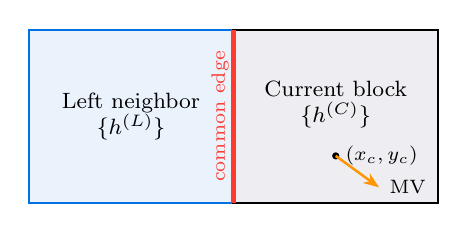
\begin{tikzpicture}[x=1cm,y=1cm]
    \draw[fill=avbluesoft, draw=avblue, line width=0.7pt] (0,0) rectangle (2.6,2.2);
    \draw[fill=avgraysoft, draw=black, line width=0.7pt] (2.6,0) rectangle (5.2,2.2);
    \draw[avred, line width=1.6pt] (2.6,0) -- (2.6,2.2);
    \node[font=\footnotesize, align=center] at (1.3,1.1) {Left neighbor\\$\{h^{(L)}\}$};
    \node[font=\footnotesize, align=center] at (3.9,1.25) {Current block\\$\{h^{(C)}\}$};
    \fill (3.9,0.6) circle (1.3pt) node[right, font=\scriptsize] {$(x_c,y_c)$};
    \draw[-{Stealth[length=2mm]}, avorange, line width=0.9pt] (3.9,0.6) -- ++(0.55,-0.4) node[right, font=\scriptsize, black] {MV};
    \node[font=\scriptsize, avred, rotate=90] at (2.43,1.1) {common edge};
  \end{tikzpicture}
  \caption{Warp extend from a left neighbor. The current block's model is
  chosen so that its motion matches the neighbor's motion along the common
  edge (red) and equals the signaled MV at the block center.}
  \label{fig:warp_extend}
\end{figure}

Consider a warped left neighbor, as in Fig.~\ref{fig:warp_extend}, with
parameters $h^{(L)}$, and let $h^{(C)}$ be the parameters of the current
block. On the common edge, the horizontal position $x$ is fixed and $y$
varies. Condition~1 requires
\begin{equation}
  \begin{bmatrix} h^{(C)}_{11} & h^{(C)}_{12} \\ h^{(C)}_{21} & h^{(C)}_{22}\end{bmatrix}
  \begin{bmatrix} x \\ y \end{bmatrix} +
  \begin{bmatrix} h^{(C)}_{13} \\ h^{(C)}_{23}\end{bmatrix} =
  \begin{bmatrix} h^{(L)}_{11} & h^{(L)}_{12} \\ h^{(L)}_{21} & h^{(L)}_{22}\end{bmatrix}
  \begin{bmatrix} x \\ y \end{bmatrix} +
  \begin{bmatrix} h^{(L)}_{13} \\ h^{(L)}_{23}\end{bmatrix}
\end{equation}
for every $y$ on the edge. Matching the coefficients of $y$ gives
$h^{(C)}_{12} = h^{(L)}_{12}$ and $h^{(C)}_{22} = h^{(L)}_{22}$; matching the
remaining terms gives
$h^{(C)}_{11}x + h^{(C)}_{13} = h^{(L)}_{11}x + h^{(L)}_{13}$ and
$h^{(C)}_{21}x + h^{(C)}_{23} = h^{(L)}_{21}x + h^{(L)}_{23}$.
Condition~2 adds $h^{(C)}_{11}x_c + h^{(C)}_{13} = \mathrm{MV}_x$ and
$h^{(C)}_{21}x_c + h^{(C)}_{23} = \mathrm{MV}_y$. Solving these equations gives
\begin{align}
  h^{(C)}_{11} &= \frac{\mathrm{MV}_x - \big(h^{(L)}_{11}x + h^{(L)}_{13}\big)}{x_c - x}, &
  h^{(C)}_{13} &= \mathrm{MV}_x - h^{(C)}_{11}x_c, \\
  h^{(C)}_{21} &= \frac{\mathrm{MV}_y - \big(h^{(L)}_{21}x + h^{(L)}_{23}\big)}{x_c - x}, &
  h^{(C)}_{23} &= \mathrm{MV}_y - h^{(C)}_{21}x_c .
\end{align}
For a neighbor above the block, the same derivation applies with the roles of
$x$ and $y$ swapped. Warp extend is a cheap way to propagate a warp model
across many blocks: each block only pays for an MV. Warp-mv and warp extend
cannot be used together in the same block.

\subsubsection{Compound Warp Causal Mode}
In AV1, the least-squares (causal) warp mode works only with single
prediction. AV2 extends it to compound prediction: a warp model is estimated
separately for each of the two references, the two warped predictions are
formed, and they are averaged. This mode is allowed only with
\code{NEW\_NEWMV}, where both MVs are explicitly coded.

\subsubsection{Generating the Warped Prediction}
AV2 supports much larger warp models than the limit in~\eqref{eq:warp_valid},
by choosing the prediction method according to the size of the model, as
shown in Algorithm~\ref{alg:warp_filter}.

\begin{algorithm}[t]
\caption{Selection of the warped prediction method}
\label{alg:warp_filter}
\DontPrintSemicolon
\KwIn{shear parameters $\alpha,\beta,\gamma,\delta$ of the block}
\KwOut{prediction method}
\uIf{$4|\alpha| + 7|\beta| < 1$ \textbf{and} $4|\gamma| + 4|\delta| < 1$}{
  shear-based 8-tap warp filter (as in AV1)\;}
\uElseIf{$4|\alpha| + 7|\beta| < 3$ \textbf{and} $4|\gamma| + 4|\delta| < 3$}{
  shear-based warp filter with short taps near the block boundary\;}
\Else{
  $4{\times}4$ sub-block translational prediction\;}
\end{algorithm}

For moderate models, AV2 keeps the shear-based filter but uses shorter filter
taps at the boundary of the predicted block, so that an $8{\times}8$
prediction still reads no more than a $15{\times}15$ reference area. For large
models, the block is split into $4{\times}4$ sub-blocks. Each sub-block gets a
translational MV from the warp model at its center $(x_c,y_c)$,
\begin{align}
  \mathrm{MV}_x &= (h_{11}-1)\,x_c + h_{12}\,y_c + h_{13}, \\
  \mathrm{MV}_y &= h_{21}\,x_c + (h_{22}-1)\,y_c + h_{23},
\end{align}
and is predicted with a 64-phase 6-tap interpolation filter. Short-tap and
$4{\times}4$ prediction would increase memory bandwidth, so AV2 groups the
sub-blocks into $8{\times}8$ units, each of which prefetches a fixed
$15{\times}15$ area; samples outside this area are padded. The worst-case
bandwidth is thus the same as in AV1.

\subsection{Wedge and Implicit Wedge Modes}
\label{sec:wedge}

\subsubsection{Parametric Wedge Masks}
A wedge mode blends two predictors with a mask that splits the block along a
straight line, which helps at object boundaries where each side of the block
follows a different motion. AV1 provides 16 hand-designed masks per block
size. AV2 instead defines the masks with a formula~\cite{av2wedge}. A straight
line is written in Hessian normal form,
\begin{equation}
  d(x,y) = x\cos\varphi - y\sin\varphi + \rho ,
  \label{eq:wedge_cont}
\end{equation}
where $\varphi$ is the angle of the line and $\rho$ is its offset from the
block center (Fig.~\ref{fig:wedge}); $d(x,y)$ is the signed distance of
$(x,y)$ from the line. The angle is quantized to 20 values in $[0,2\pi)$,
chosen by their tangent so that they fit blocks of different aspect ratios,
and the offset is quantized to a few values based on the block width or
height. As shown in Fig.~\ref{fig:wedge}, 8 angles are used with 4 offsets
(32 modes) and 12 angles with 3 offsets (36 modes), for up to 68 wedge modes
per block size.

\begin{figure}[t]
  \centering
  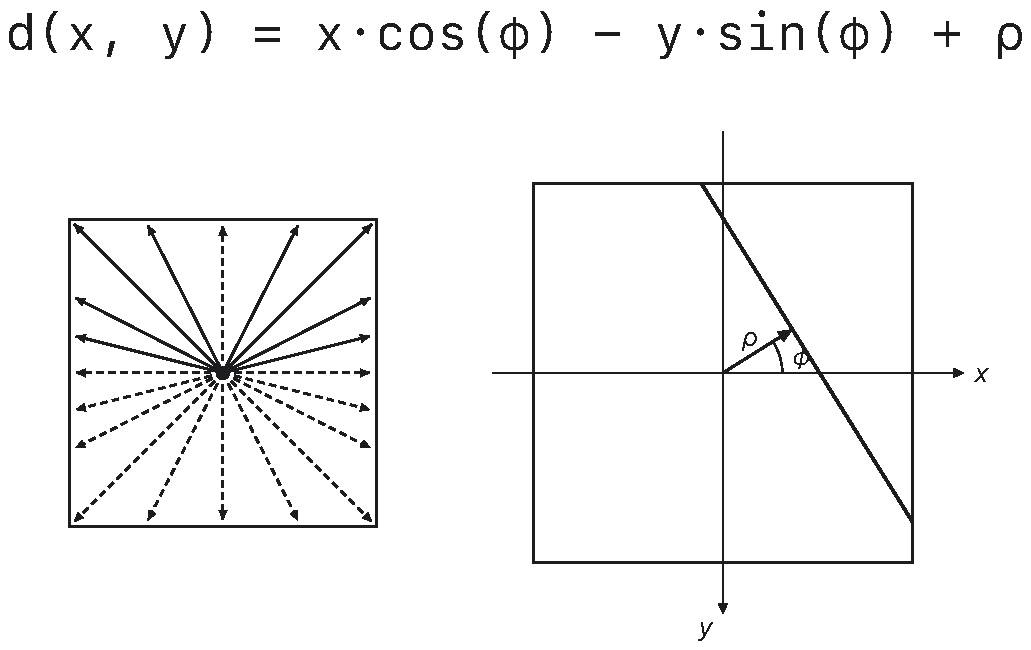
\includegraphics[width=0.72\columnwidth]{figures/wedge.pdf}
  \caption{Parametric wedge masks in AV2. The boundary is a line at angle
  $\varphi$ and offset $\rho$ from the block center. Solid lines: 8 angles
  with 4 offsets each (32 modes); dashed lines: 12 angles with 3 offsets each
  (36 modes).}
  \label{fig:wedge}
\end{figure}

For hardware, the cosine and sine are replaced by lookup tables (LUTs) that contain
only $0$ and powers of two, so that the distance becomes a sum of shifts. For
a $w\times h$ block and quantized angle index $i$ and offset index $j$, the
distance of sample $(m,n)$ is
\begin{equation}
  \begin{aligned}
  d(m,n) ={} & \big(2(m+\rho_{j,m}) - w + 1\big)\,\mathrm{COSLUT}(i) \\
             & + \big(2(n+\rho_{j,n}) - h + 1\big)\,\mathrm{SINLUT}(i),
  \end{aligned}
  \label{eq:wedge_disc}
\end{equation}
where $\mathrm{COSLUT}(\cdot)$ and $\mathrm{SINLUT}(\cdot)$ are the cosine and
sine LUTs, and $\rho_{j,m}$ and $\rho_{j,n}$ are the horizontal and vertical
parts of the offset. The mask weight is a smooth function of the distance,
$\omega(m,n) = f\big(d(m,n)\big)$. AV2 uses a sigmoid,
\begin{equation}
  \omega(m,n) = \frac{1}{1+e^{-2d(m,n)}},
  \label{eq:sigmoid}
\end{equation}
which gives a sharp but not abrupt transition and so preserves edges. In the
codec the sigmoid is tabulated with integer weights. Two blending widths are
used, chosen implicitly from the block size.

\subsubsection{Implicit Wedge Mode (IWM)}
When an MV points partly outside the reference picture, the samples outside
the picture are made by repeating the border samples. Such samples are poor
predictions. In compound prediction it often happens that one predictor is
inside the picture where the other is outside, for example when the camera
pans. IWM handles this case automatically (Fig.~\ref{fig:iwm}). For each
sample, the decoder checks whether each of the two reference positions is
inside the reference picture. If both are inside, or both are outside, the
weights (out of 64) are $(32,32)$, i.e., normal averaging. If only one is
inside, that predictor gets weight 64 and the other gets 0.
IWM is applied when at least one predictor of a compound block is partly or
fully outside the picture. It needs no signaling.

\begin{figure}[t]
  \centering
  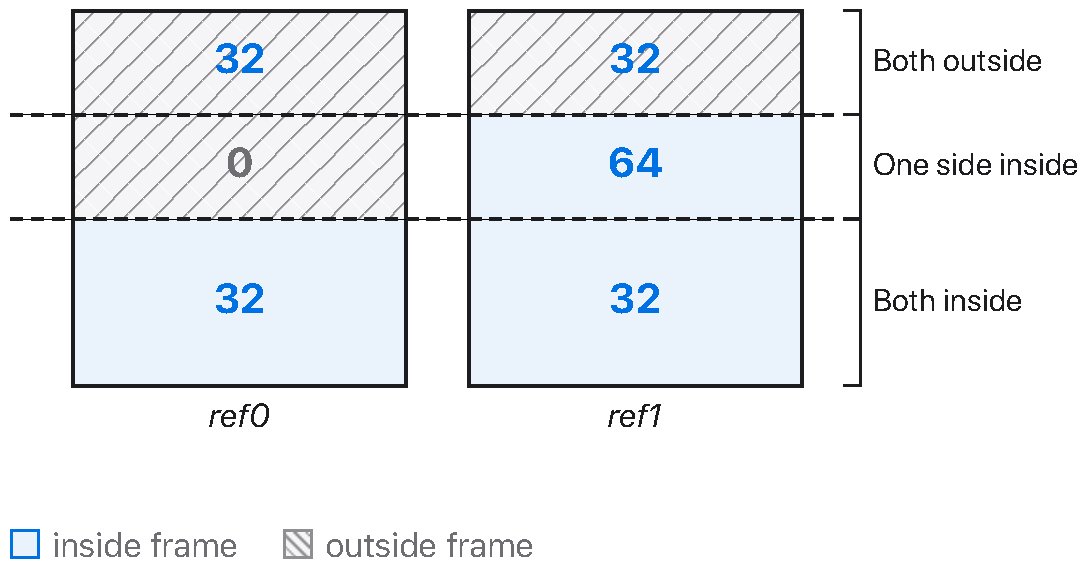
\includegraphics[width=0.62\columnwidth]{figures/iwm.pdf}
  \caption{Implicit wedge mode. Hatched areas of a reference block lie
  outside the reference picture. Numbers are the blending weights (out of
  64). Where only one predictor is inside the picture, that predictor gets all
  the weight.}
  \label{fig:iwm}
\end{figure}

\subsection{Weighted Prediction}
\label{sec:weighted}

\subsubsection{Compound Weighted Prediction (CWP)}
Simple averaging is optimal only if both predictors are equally good. CWP
lets the encoder choose an unequal weight for \code{COMPOUND\_AVERAGE}
blocks:
\begin{equation}
  P(x,y) = \big(W\,P_0(x,y) + (16-W)\,P_1(x,y) + 8\big) \gg 4,
  \label{eq:cwp}
\end{equation}
where $\gg$ is a right shift. When the two references are on opposite sides,
$W\in\{8,10,6,12,4\}$. When they are on the same side,
$W\in\{8,12,4,20,-4\}$; here weights outside $[0,16]$ allow linear
extrapolation, which matches motion and brightness trends that continue in
time. The weight index is signaled only when the compound type is
\code{COMPOUND\_AVERAGE}, the mode is \code{NEAR\_NEARMV}, \code{JOINT\_NEWMV},
or \code{JOINT\_AMVDNEWMV}, and, for joint MVD modes, the MVD scaling is the
identity (Section~\ref{sec:jmvd}). In skip mode, the weight index is not
signaled; it is inherited from the neighbor that provided the selected DRL
candidate.

\subsubsection{Block Adaptive Weighted Prediction (BAWP)}
Brightness changes, such as fades, flashes, or a light switched on in part of
the scene, make even a perfectly aligned reference block look different from
the current block. BAWP~\cite{inter_bacp} corrects this with a linear model
per color component,
\begin{equation}
  P'(x,y) = \alpha\,P(x,y) + \beta ,
  \label{eq:bawp}
\end{equation}
where $P$ is the regular inter prediction. The offset $\beta$ is always
derived at the decoder. The scale $\alpha$ is either derived at the decoder
(implicit BAWP) or signaled (explicit BAWP).

For the implicit derivation, the current block has an L-shaped template of
already reconstructed samples above and to the left of it. The reference
block, located with the integer part of the MV, has a template at the same
relative position. Let $\{r_k\}$ and $\{c_k\}$, $k=1,\ldots,N$, be the
reference-template and current-template samples. The decoder fits the model
so that it maps the reference template onto the reconstructed template with
the smallest squared error,
\begin{equation}
  (\alpha^{*},\beta^{*}) = \arg\min_{\alpha,\beta}\ \sum_{k=1}^{N}\big(c_k - \alpha r_k - \beta\big)^2 ,
\end{equation}
whose solution is
\begin{equation}
  \alpha = \frac{N\sum r_k c_k - \sum r_k \sum c_k}{N\sum r_k^2 - \big(\sum r_k\big)^2},
  \qquad
  \beta = \frac{\sum c_k - \alpha\sum r_k}{N},
  \label{eq:bawp_ls}
\end{equation}
which the codec evaluates with integer arithmetic. With explicit $\alpha$,
only $\beta$ is computed from~\eqref{eq:bawp_ls}. Three choices keep BAWP
cheap. Only the first row and the first column of the template are used,
with at most 8 samples, so the fit is a few multiply-accumulate operations.
The integer MV avoids interpolating the template. And the luma $\alpha$ is
reused for both chroma components, while each chroma component derives its
own $\beta$; this reduces computation for implicit BAWP and signaling for
explicit BAWP.

%% =============================================================================
\section{Motion Vector Prediction}
\label{sec:mvpred}
%% =============================================================================

MVs take a large share of the bit rate, especially at low rates, so the
quality of the MV predictor matters a lot. AV2 builds its DRL from several
sources (Fig.~\ref{fig:drl}): spatial MV prediction (SMVP) from adjacent
neighbors, temporal MV prediction (TMVP) from the projected motion field, non-adjacent spatial
neighbors, the reference MV bank, candidates derived from combinations of
other candidates, and the global motion model. The candidates are ranked, and
the encoder signals the index of the one it uses. Below we describe the
sources and then the ranking.

\begin{figure*}[t]
  \centering
  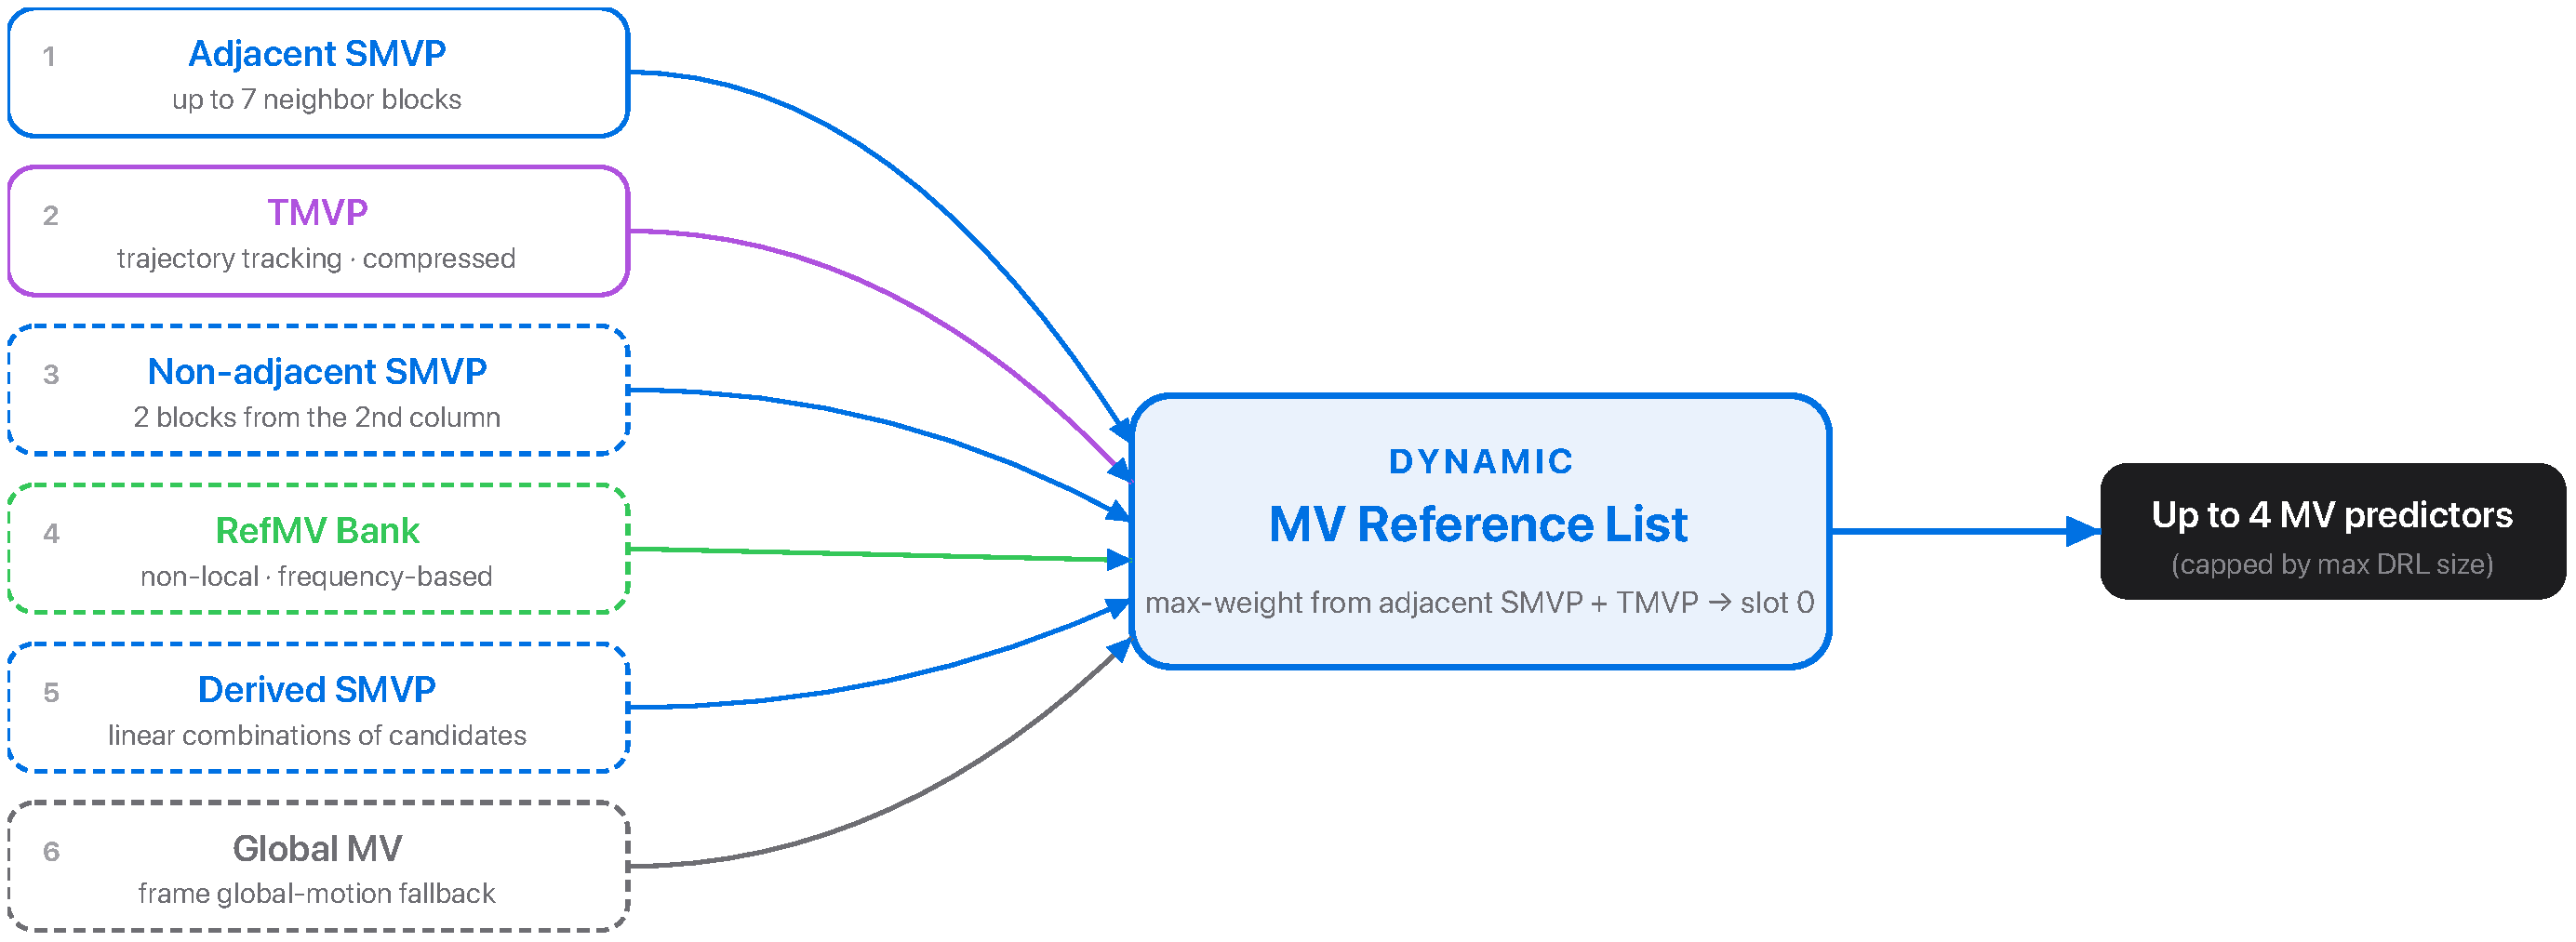
\includegraphics[width=0.70\textwidth]{figures/drl.pdf}
  \caption{Sources of the dynamic MV reference list (DRL) in AV2. The adjacent
  spatial candidates and the temporal candidate are ranked first by their
  weights; the other sources fill the rest of the list, which has at most
  four predictors.}
  \label{fig:drl}
\end{figure*}

\subsection{Spatial MV Prediction}
\label{sec:smvp}
The spatial neighbors of the current block are checked for blocks that use the
same reference frame (for compound blocks, the same pair of references). AV2
simplifies the AV1 search, which scanned up to three block rows above and
three block columns to the left. AV2 checks up to nine neighbors in the fixed
order shown in Fig.~\ref{fig:spatial_scan}. Positions 1--7 are adjacent to the
block; positions 8 and 9 are in the second column to the left. The first six
distinct MVs found are recorded together with an occurrence count (weight)
and a flag that tells whether they come from the nearest row or column.

\begin{figure}[t]
  \centering
  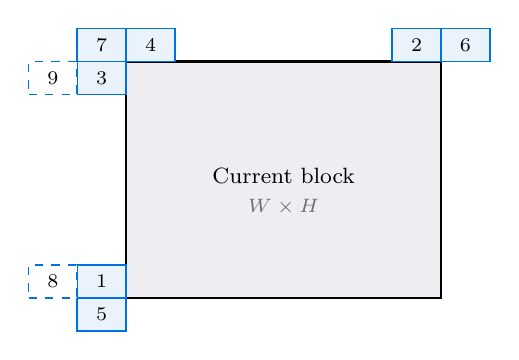
\begin{tikzpicture}[x=1cm,y=1cm,
      nb/.style={draw=avblue, fill=avbluesoft, line width=0.6pt, minimum width=0.62cm, minimum height=0.42cm, font=\scriptsize, inner sep=0pt},
      far/.style={nb, fill=white, dashed}]
    % current block
    \draw[line width=0.8pt, fill=avgraysoft] (0,0) rectangle (4,3);
    \node[font=\footnotesize] at (2,1.55) {Current block};
    \node[font=\scriptsize, avgray] at (2,1.15) {$W \times H$};
    % adjacent neighbors (nearest row and column)
    \node[nb] at (-0.31,0.21) {1};
    \node[nb] at ( 3.69,3.21) {2};
    \node[nb] at (-0.31,2.79) {3};
    \node[nb] at ( 0.31,3.21) {4};
    \node[nb] at (-0.31,-0.21) {5};
    \node[nb] at ( 4.31,3.21) {6};
    % top-left corner
    \node[nb] at (-0.31,3.21) {7};
    % non-adjacent neighbors (second column)
    \node[far] at (-0.93,0.21) {8};
    \node[far] at (-0.93,2.79) {9};
  \end{tikzpicture}
  \caption{Spatial neighbor positions and checking order used for SMVP (and
  reused by the WRL). Positions 1--6 are on the nearest row and column,
  position 7 is the top-left corner, and positions 8 and 9 (dashed) are
  non-adjacent blocks in the second column.}
  \label{fig:spatial_scan}
\end{figure}

The search region was chosen with the hardware line buffer in mind. A hardware
decoder processes the frame one superblock at a time, in raster order. Motion
information of the row of blocks just above the current superblock row has to
be kept in a \emph{line buffer}, an on-chip memory whose size is set by the
widest frame allowed. Since the smallest block in AV2 is $4{\times}4$, storing
MVs at $4{\times}4$ granularity for a whole frame width is expensive. AV2
therefore reads only the even-indexed $4{\times}4$ units (counting from 0) of
the last row of the superblock above, which halves the line buffer. Inside the
current superblock, all $4{\times}4$ units can be used, because that
information is in local memory anyway. The left context depends only on the
superblock size, so its cost is small, but AV2 uses the same subsampling on the
left as above so that the ranking does not favor one side.

\subsection{Temporal MV Prediction (TMVP)}
\label{sec:tmvp}
TMVP predicts the MVs of the current frame from the MVs stored with
previously decoded frames. As in AV1, a motion field is built for the current
frame before it is decoded: stored MVs are projected along their motion
direction onto the current frame, and every $8{\times}8$ block of the current
frame that a projected MV lands in gets a motion field MV~\cite{MVref}. The
motion field is used for TMVP candidates and by TIP. AV2 improves this process
in three ways.

\subsubsection{Motion Projection Order}
The stored MVs of different reference frames are not equally useful. AV2
orders the projection by temporal distance, which is a good proxy for
correlation. Nearby past and future references whose MVs point towards the
current frame are processed first, in order of priority. Then the motion
fields of the two closest past references whose MVs point away from the
current frame are used. The process stops once three motion fields have been
collected, which bounds the projection work.

\subsubsection{MV Trajectory Tracking}
AV1 projects a single stored MV along a straight line
(Fig.~\ref{fig:tmvp_traj}(a)). This fails when the motion is not linear, for
example for objects on curved paths, for accelerating objects, or for camera
shake. AV2 instead follows motion trajectories over several references
(Fig.~\ref{fig:tmvp_traj}(b)). It keeps a two-way mapping between blocks of
the current frame and blocks of the reference frames. When a stored MV starts
or ends at a block that is already on a trajectory, the MV is appended to that
trajectory. Chaining MVs in this way approximates the real, curved path of the
object much better than a single straight-line projection.

\begin{figure*}[t]
  \centering
  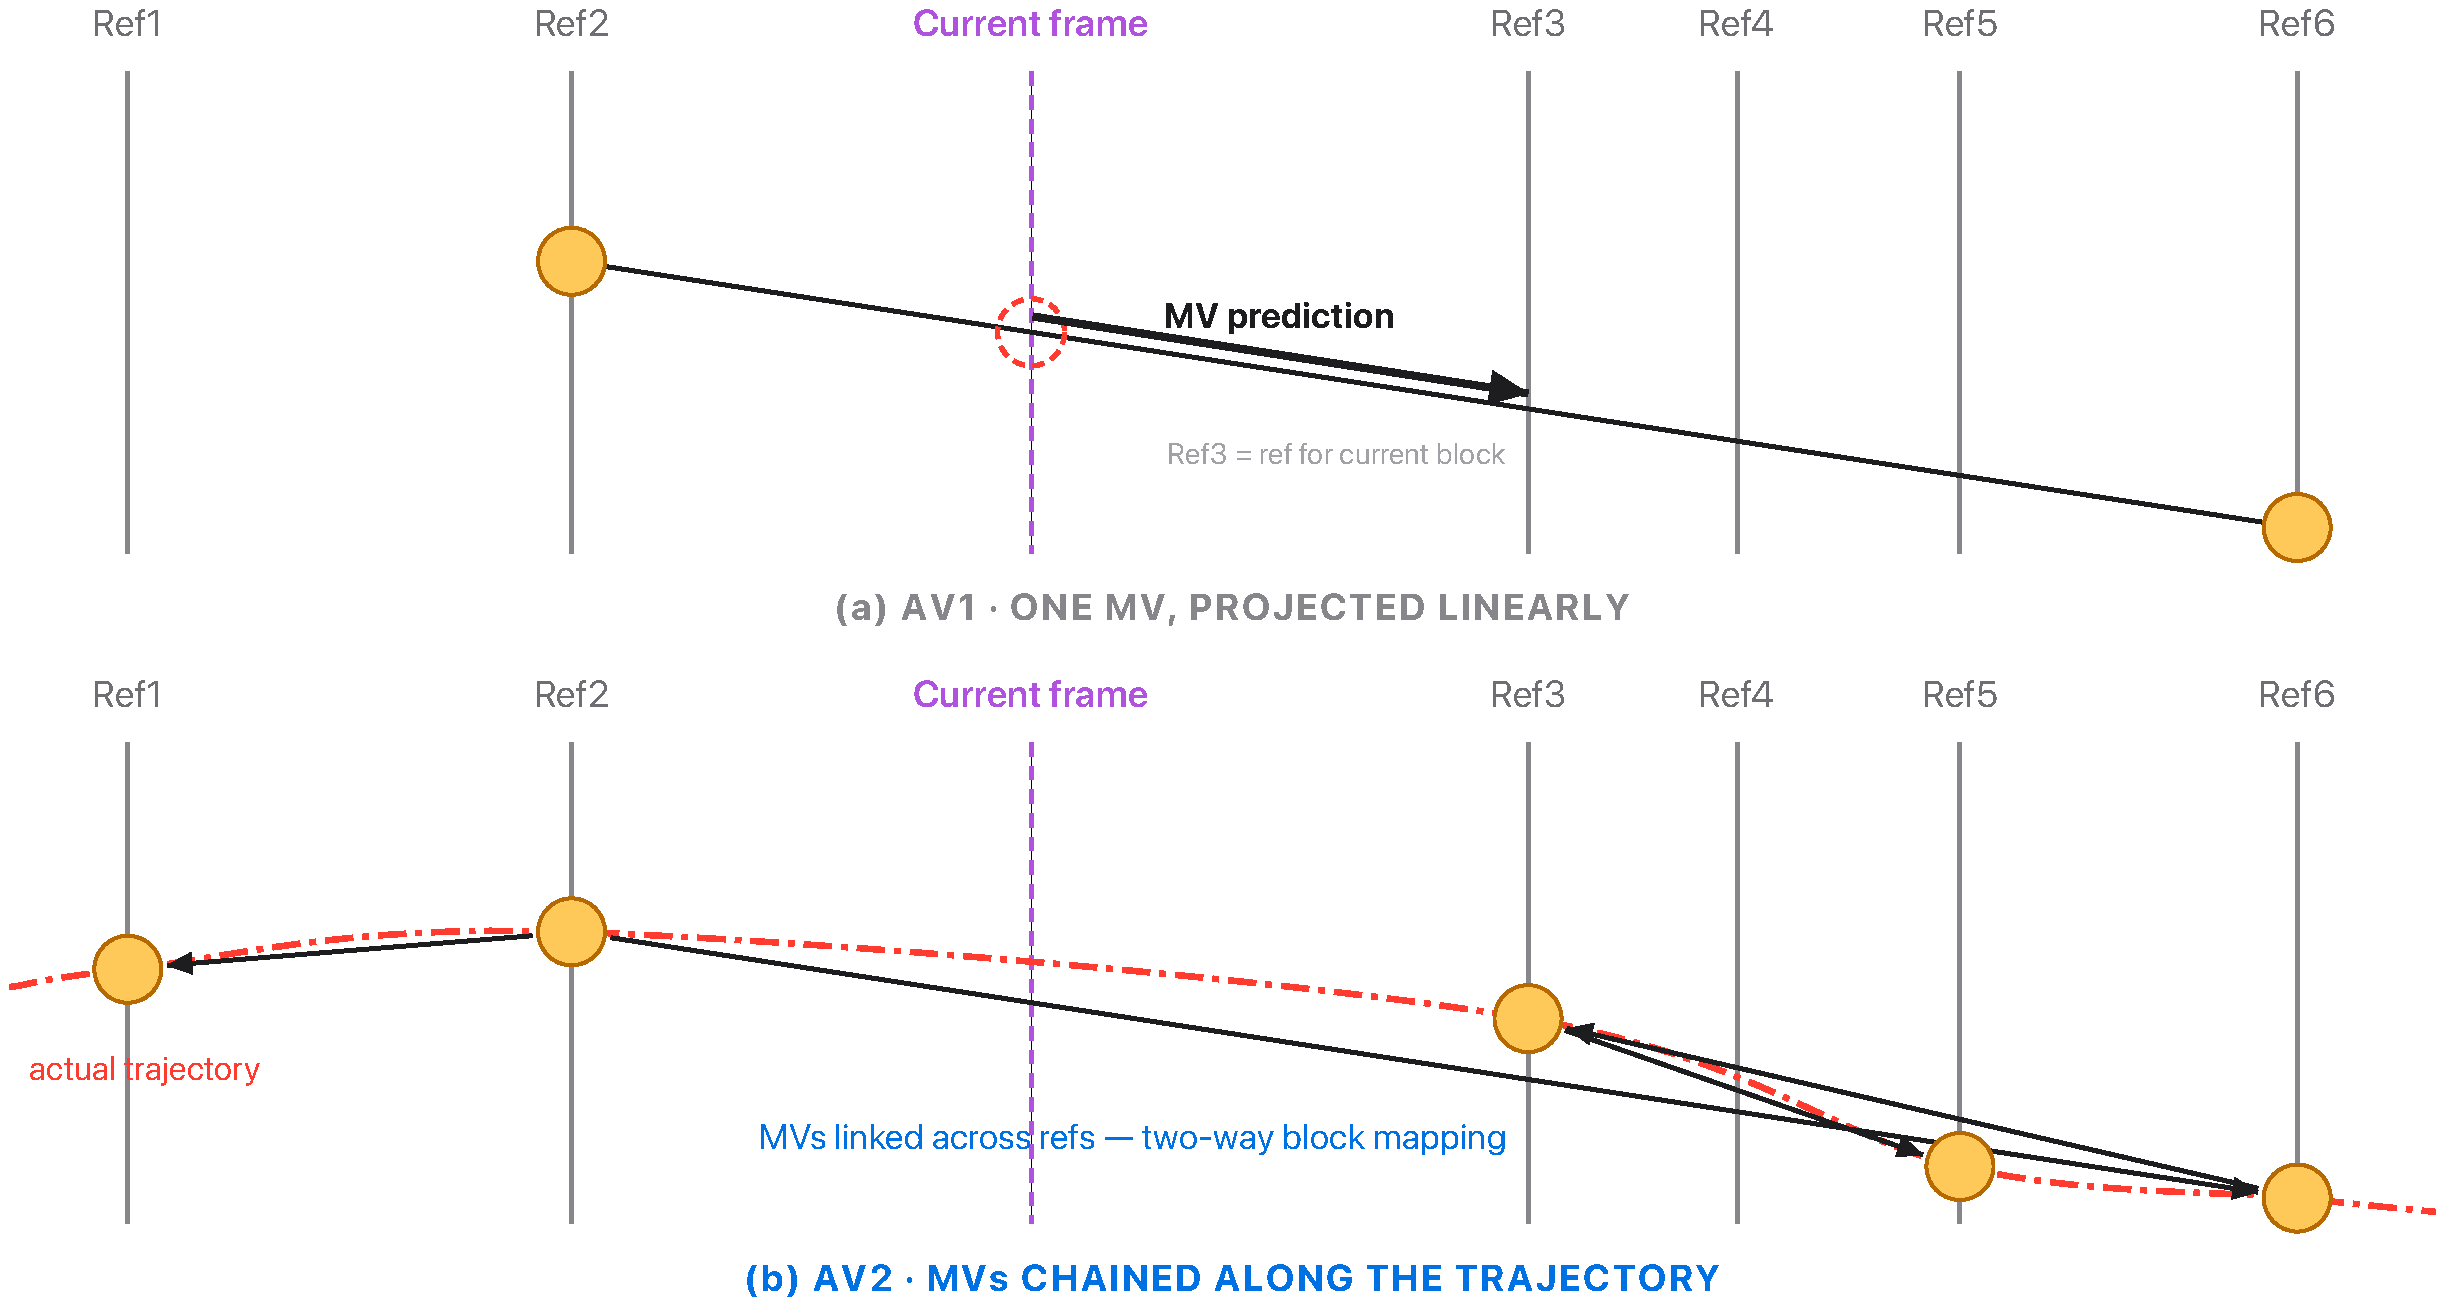
\includegraphics[width=0.62\textwidth]{figures/tmvp_traj.pdf}
  \caption{TMVP with (a) linear projection in AV1, where one stored MV is
  extended in a straight line across the current frame, and (b) trajectory
  tracking in AV2, where MVs of several references are chained along the
  object's actual (curved) path using two-way block mappings.}
  \label{fig:tmvp_traj}
\end{figure*}

\subsubsection{Memory Reduction}
Stored MVs live in external memory and must be read for every frame that
references them, so their size directly sets memory bandwidth. AV2 reduces
this cost with three techniques.

\emph{MV compression.} In AV1, a stored MV takes 26 bits: two components, each
with a sign and 12 magnitude bits. AV2 stores 16 bits per MV
(Fig.~\ref{fig:tmvp_comp}). First, one magnitude bit per component is dropped,
so magnitudes are limited to $[0, 2047]$ (larger MVs are discarded). Second,
the 11-bit magnitude is quantized to a 7-bit index with eight bins: values up
to 31 are kept exactly, and larger values are quantized with step sizes that
double from bin to bin ($2, 4, \ldots, 64$). This keeps full precision for
small MVs, which are the most common, and loses only relative precision for
large ones. The mapping needs only shifts.

\begin{figure*}[t]
  \centering
  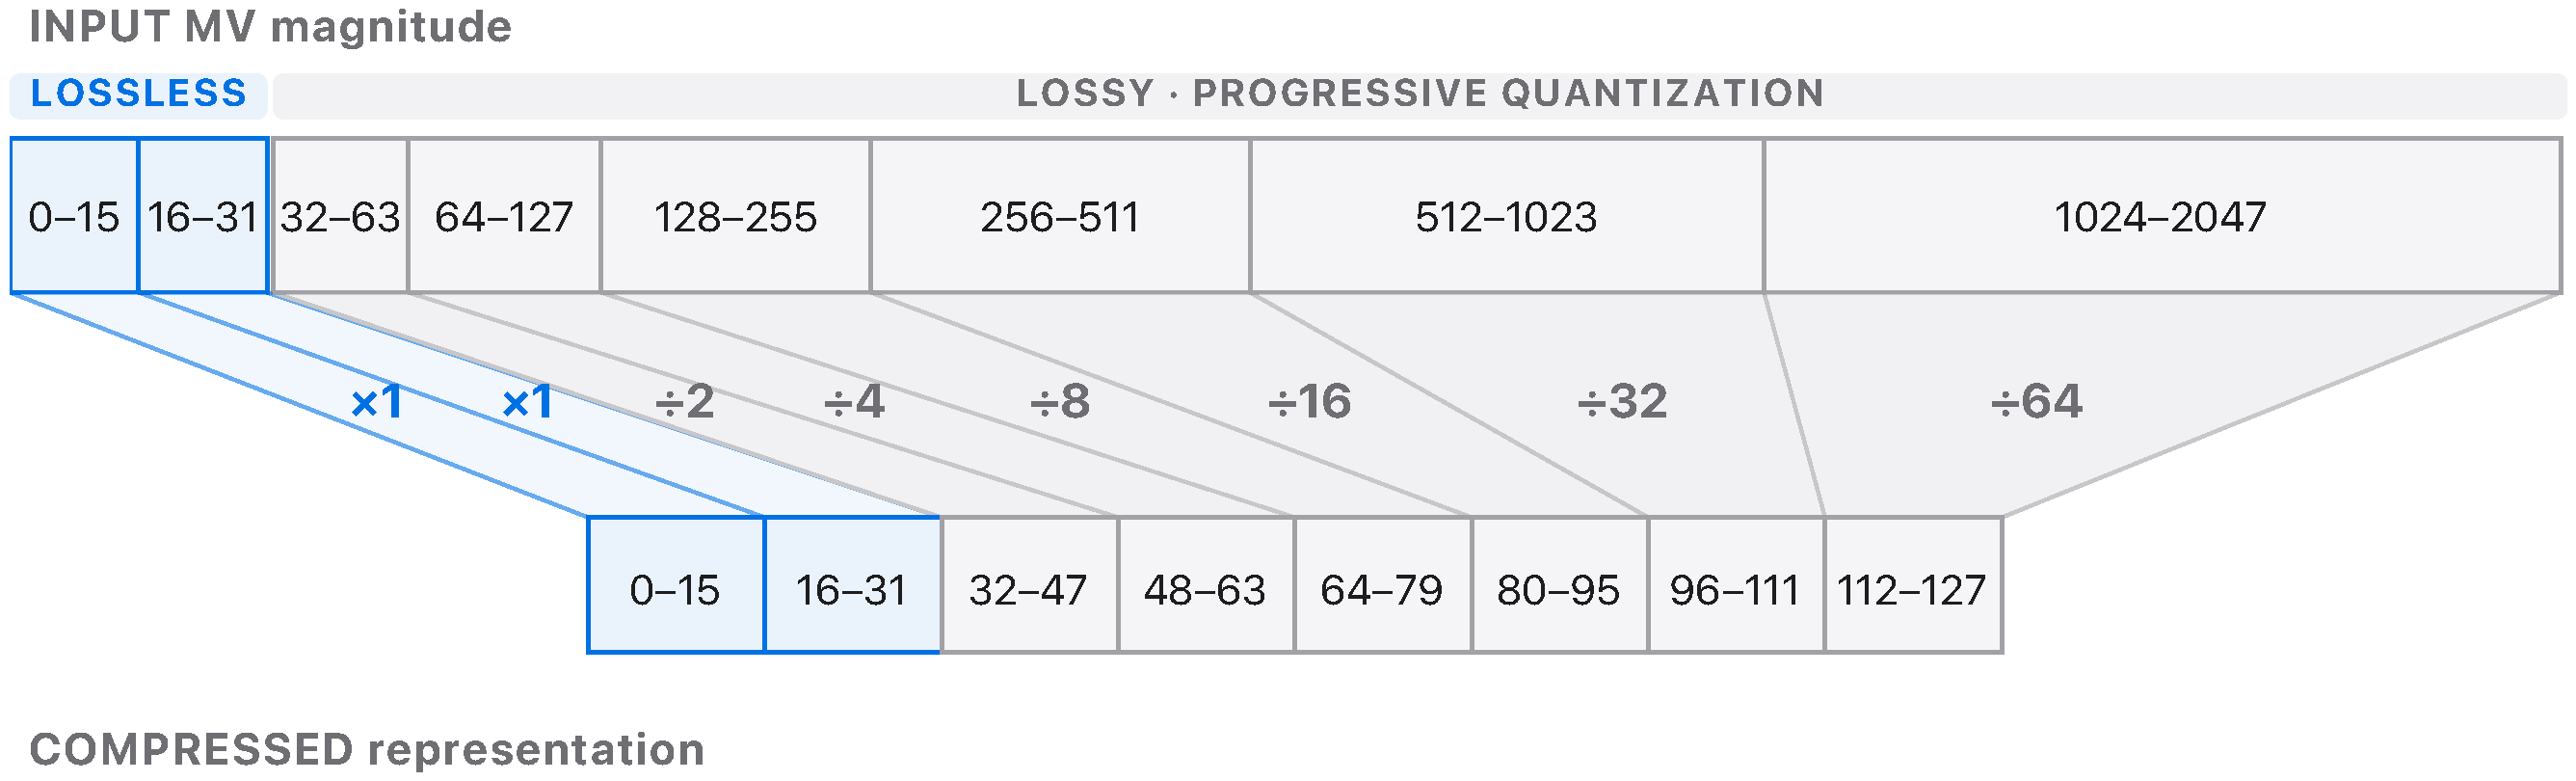
\includegraphics[width=0.72\textwidth]{figures/tmvp_comp.pdf}
  \caption{Compression of stored MVs for TMVP from 26 to 16 bits. After one
  bit per component is dropped, the 11-bit magnitude is mapped to a 7-bit
  index: the first two bins are lossless, and the remaining bins are quantized
  with step sizes $2,4,\ldots,64$.}
  \label{fig:tmvp_comp}
\end{figure*}

\emph{Directional storage.} Each $8{\times}8$ block of a reference frame can
store two MVs. Usually only one of them is useful for a given current frame,
namely the one that points towards it. AV2 assigns the two slots by
direction, one for an MV pointing to the past and one for an MV pointing to
the future, so a decoder can load only the slot it needs.

\emph{Adaptive sampling.} Only stored MVs within a limited window around the
collocated area can be used, which bounds the memory a hardware decoder must
hold. A larger window covers larger motion but needs more memory. AV2 lets the
codec use either a small window with all MVs, or a larger window with 1:4
subsampled MVs. The first suits slow motion, where precision matters; the
second suits fast motion, where coverage matters.

\subsection{Reference MV Bank}
\label{sec:bank}
Spatial candidates come only from the immediate neighborhood. Good predictors
are often found farther away, for example on the same object a few blocks to
the left. The reference MV bank~\cite{av2spec} makes such non-local MVs
available without complex search rules or large memory.

\begin{figure}[t]
  \centering
  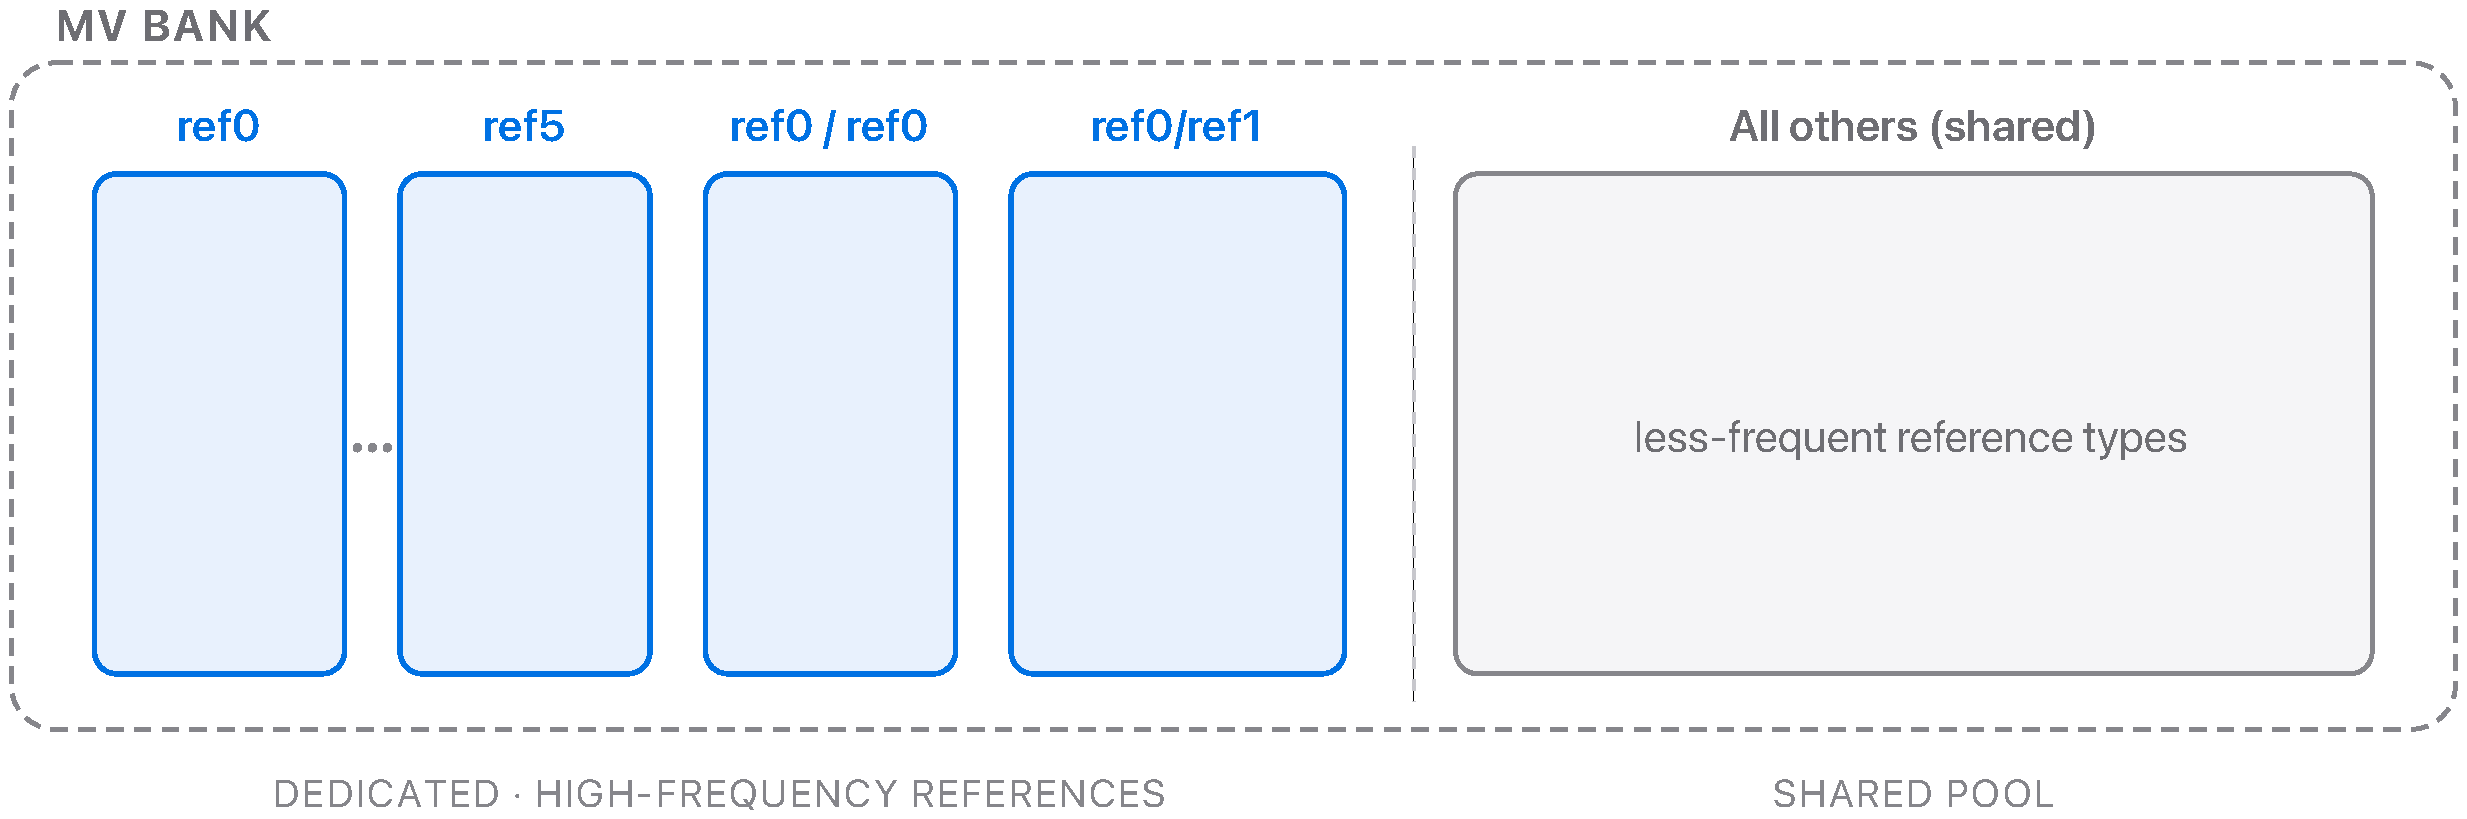
\includegraphics[width=0.98\columnwidth]{figures/mv_bank.pdf}
  \caption{Frequency-based reference MV bank. The most frequently used single
  and compound reference types have dedicated buffers; all other reference
  types share one buffer.}
  \label{fig:mv_bank}
\end{figure}

The bank is a set of small buffers. A buffer for every possible reference type
(each single reference and each compound pair) would be large, so AV2 uses a
frequency-based design (Fig.~\ref{fig:mv_bank}): the most frequently used
reference types get their own buffers, and the less frequent types share one
buffer. After an inter block is decoded, its MV is added to the buffer of its
reference type: an MV not yet in the buffer is appended at the end, and an MV
already in the buffer is moved to the end. The end of the buffer thus always
holds the most recently used MVs, as in a least-recently-used cache. To bound
hardware cost, at most 64 updates are made per superblock, and the bank is
reset at the start of each superblock row, which keeps superblock rows
independent for parallel decoding. When the DRL is not full after the spatial
and temporal candidates, entries are taken from the end of the bank, most
recent first.

\subsection{DRL Construction}
\label{sec:drl}
The candidates are split into two groups. Group~1 contains the adjacent
spatial candidates (positions 1--7 in Fig.~\ref{fig:spatial_scan}) and the
TMVP candidate. Group~2 contains everything else: non-adjacent spatial
candidates, bank entries, derived candidates, and the global motion
candidate. Group~1 is ranked by weight, where a candidate that occurs more
often nearby is considered more likely, and is then followed by Group~2. The
first four entries form the DRL; the candidate with the largest weight from
Group~1 always takes the first slot. If fewer candidates are available, the
list is shorter, which saves bits for the index. The encoder sends the index
of the selected predictor.
\authnote{Please add one or two sentences on how non-adjacent and derived
SMVP candidates are formed.}

For each block, AV2 signals whether the selected predictor is used as is or
whether an MVD follows. For compound modes, this gives four cases depending on
which of the two MVs has a non-zero MVD (for example \code{NEAR\_NEARMV},
\code{NEW\_NEARMV}, \code{NEAR\_NEWMV}, and \code{NEW\_NEWMV}).

%% =============================================================================
\section{Motion Vector Coding}
\label{sec:mvcoding}
%% =============================================================================

After prediction, the MVD is entropy coded~\cite{MVpred-RD,MVpred-hevc}. AV2
changes MV coding in four ways: a larger MV range, flexible MV precision,
adaptive and joint MVD coding, and a new MVD entropy coder.

\subsection{MV Range Extension}
To handle very large motion, for example at 8K resolution or in fast sports
content, AV2 extends the range of MVs and MVDs from 15 to 17
bits~\cite{MV-range-extension}, while keeping $1/8$-pel precision. The
full-pel MV range becomes 14 bits, from $-2^{13}$ to $2^{13}-1$ pels.

\subsection{Flexible MV Resolution (FMVR)}
\label{sec:fmvr}
A more precise MV gives a better prediction but costs more bits. In a smooth,
slow region $1/8$-pel precision pays off; in a fast, blurry region it does
not. AV1 can only choose $1/4$- or $1/8$-pel precision per frame. AV2 adds
$1/2$-pel to the frame-level choice (a ternary flag) and, more importantly,
lets each block choose its own precision~\cite{fmvr}, within a set determined
by the frame-level maximum (Table~\ref{tab:fmvr}). The block precision is sent
before the MVD: one flag says whether the block uses the frame precision, and
if not, a further symbol selects one of the other allowed values.

\begin{table}[t]
\centering
\caption{Allowed block-level MV precisions (in pels) for each frame-level maximum precision.}
\label{tab:fmvr}
\renewcommand{\arraystretch}{1.15}
\begin{tabular}{@{}cc@{}}
\toprule
\textbf{Frame maximum precision} & \textbf{Allowed block precisions} \\
\midrule
$1/8$ & $1/8,\ 1/2,\ 1,\ 4$ \\
$1/4$ & $1/4,\ 1,\ 4,\ 8$ \\
$1/2$ & $1/2,\ 1,\ 4,\ 8$ \\
\bottomrule
\end{tabular}
\end{table}

\subsection{Adaptive MVD (AMVD) Coding}
\label{sec:amvd}
In AV1 the MVD has the same precision regardless of its size. But a large MVD
usually means the predictor was poor, and for such a block a very precise
correction is not worth its cost. AMVD~\cite{av2amvd} ties the precision to the
magnitude: small MVDs are coded at fine precision and large ones at coarse
precision. In AMVD modes, the MVD magnitude (in $1/8$ pel) is restricted to
the set $\{0, 2, 4, 6, 8, 16, 32, 64, 128\}$, so only a short index is coded.
AMVD is available in \code{NEWMV}, \code{NEW\_NEWMV}, \code{NEW\_NEARMV},
\code{NEAR\_NEWMV}, and \code{JOINT\_NEWMV} (as \code{AMVDNEWMV},
\code{JOINT\_AMVDNEWMV}, etc.).

\subsection{Joint MVD (JMVD) Coding}
\label{sec:jmvd}
In compound prediction, the MV errors of the two references are often related:
if the object moves at constant speed, the correction needed for one MV is a
scaled copy of the correction needed for the other. JMVD sends only one MVD,
$\mathrm{joint\_mvd}$, which is applied to the reference that is farther in
time, and derives the MVD of the other reference by scaling with the temporal
distances $d_0$ and $d_1$:
\begin{equation}
  \mathrm{derived\_mvd} = S_k\!\left(\sigma\,\frac{\min(|d_0|,|d_1|)}{\max(|d_0|,|d_1|)}\,\mathrm{joint\_mvd}\right).
  \label{eq:jmvd}
\end{equation}
Here $\sigma=-1$ if the two references are on opposite sides of the current
frame and $\sigma=+1$ if they are on the same side. $S_k$ is a scaling mode
signaled per block, chosen from the identity, doubling or halving the row
component, and doubling or halving the column component. The scaling modes
let JMVD follow motion that is not exactly linear in time. Whenever the linear model is good enough, JMVD
codes one MVD instead of two for a compound block.

\subsection{MVD Entropy Coding}
\label{sec:mvd_coding}
AV1 codes the row and the column of the MVD separately. The two components are
not independent, however: if one is large the other tends to be large too.
AV2 codes them jointly using \emph{shells}. All MVDs with the same sum of
absolute components form one shell,
\begin{equation}
  |\mvd_r| + |\mvd_c| = \mathrm{shell\_index},
  \label{eq:shell}
\end{equation}
as shown in Fig.~\ref{fig:mvd_shell}. Coding an MVD then means coding which
shell it lies on, where on the shell it lies, and the signs.

\begin{figure}[t]
  \centering
  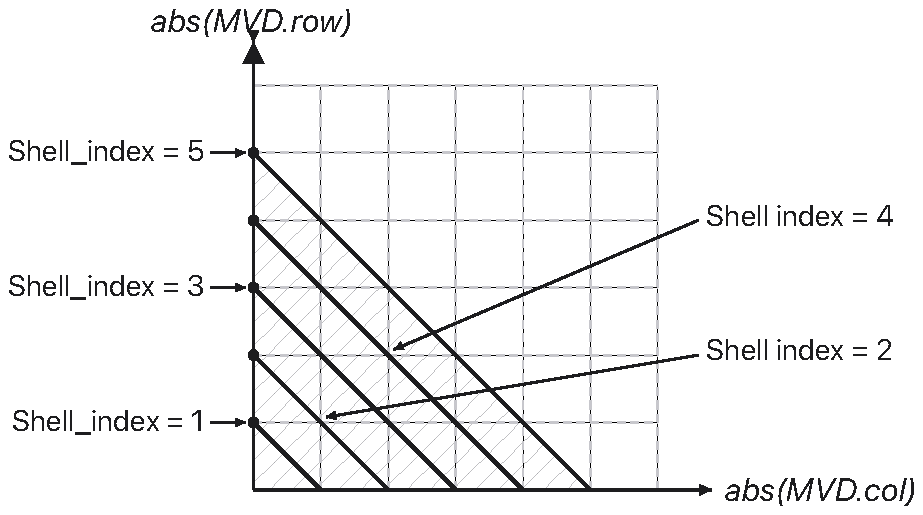
\includegraphics[width=0.64\columnwidth]{figures/mvd_shell.pdf}
  \caption{Shell representation of the MVD magnitude. All MVDs with the same
  $|\mvd_r| + |\mvd_c|$ lie on one diagonal shell.}
  \label{fig:mvd_shell}
\end{figure}

\emph{Precision normalization.} The MVD is first expressed in units of the
block precision $p$ (an integer that represents the precision, with
$p=6$ for $1/8$-pel):
\begin{equation}
  |\mathrm{scaledMVD}| = |\mvd| \gg (6 - p),
\end{equation}
for both components, and the shell index is computed from the scaled values.
This way, a coarse-precision block never spends bits on precision it cannot
use.

\emph{Shell index.} The shell index is split into a class and an offset, much
like an exponential-Golomb code. The class, $\mathrm{shell\_class}$, is coded
as one symbol with a separate probability model for each MV precision. The
offset is coded with one binary symbol if $\mathrm{shell\_class}<2$, with a
context-coded truncated unary code if $\mathrm{shell\_class}=2$, and otherwise
bit by bit, from the least to the most significant bit, with a separate
context for each bit position.

\emph{Position on the shell.} Given the shell index, $|\mvd_c|$ lies in
$[0,\mathrm{shell\_index}]$. Values near 0 are mostly vertical MVDs and values
near $\mathrm{shell\_index}$ are mostly horizontal MVDs; both are common.
AV2 therefore folds the range around its middle and, with
$s = \mathrm{shell\_index}$, codes
\begin{equation}
  \mathrm{pair\_idx} =
  \begin{cases}
    |\mvd_c|, & |\mvd_c| \le \lfloor s/2 \rfloor,\\
    s - |\mvd_c|, & \text{otherwise},
  \end{cases}
\end{equation}
followed by one bit that tells which half $|\mvd_c|$ is in (with four
contexts selected by $\min(\mathrm{shell\_class},3)$). The folded index is coded
with a ``greater than 0'' flag, a ``greater than 1'' flag (one context each),
and a quasi-uniform code for the rest. The row magnitude follows from
$|\mvd_r| = \mathrm{shell\_index} - |\mvd_c|$.

\emph{Signs.} The signs of non-zero components are coded one by one, except
that the sign of the \emph{last} non-zero component can be inferred instead
of sent. The encoder chooses the MVD so that the parity of the sum of the
(precision-scaled) magnitudes matches that sign: an odd sum means negative,
an even sum means positive. This is enabled when the number of non-zero MVD
components reaches a threshold, 4 for \code{NEW\_NEWMV} (two full MVDs) and 1
for other modes. Algorithm~\ref{alg:sign} gives the decoder side.

\begin{algorithm}[t]
\caption{Decoding the sign of the last non-zero MVD component}
\label{alg:sign}
\DontPrintSemicolon
$s \leftarrow \code{MV\_PRECISION\_EIGHTH\_PEL} - p$\;
decode the magnitudes of all MVD components\;
decode the signs of all non-zero components except the last one\;
$\mathit{sum} \leftarrow \sum_k (|\mvd_k| \gg s)$;\quad
$\mathit{nz} \leftarrow \#\{k : |\mvd_k| \ne 0\}$\;
$\mathit{thr} \leftarrow 4$ \textbf{if} mode is \code{NEW\_NEWMV} (or its OPFL variant) \textbf{else} $1$\;
\eIf{$\mathit{nz} \ge \mathit{thr}$}{
  sign of last non-zero component $\leftarrow$ negative if $\mathit{sum}$ is odd, positive otherwise\;}{
  decode the sign of the last non-zero component\;}
\end{algorithm}

%% =============================================================================
\section{Backward Reference Updating (BRU)}
\label{sec:bru}
%% =============================================================================

\subsection{Motivation}
In some applications, such as screen mirroring, remote desktop, or a drawing
app, most of the picture does not change from frame to frame. A conventional
decoder still processes the full frame: it reads the reference frame, writes a
complete new frame into the DPB, and runs the in-loop filters
everywhere (Fig.~\ref{fig:bru_motiv}). For 4K 4:2:0 8-bit video, a frame is
about 12.4\,MB, so reading and writing it costs about 25\,MB of memory traffic
per frame, or about 1.5\,GB/s at 60 frames per second, even when only a small
stroke has changed. BRU~\cite{bru} lets a decoder avoid most of this work. It
signals which superblocks are active, decodes only those, and writes them
\emph{back} into an existing reference frame in place, instead of building a
new frame.

\begin{figure*}[t]
  \centering
  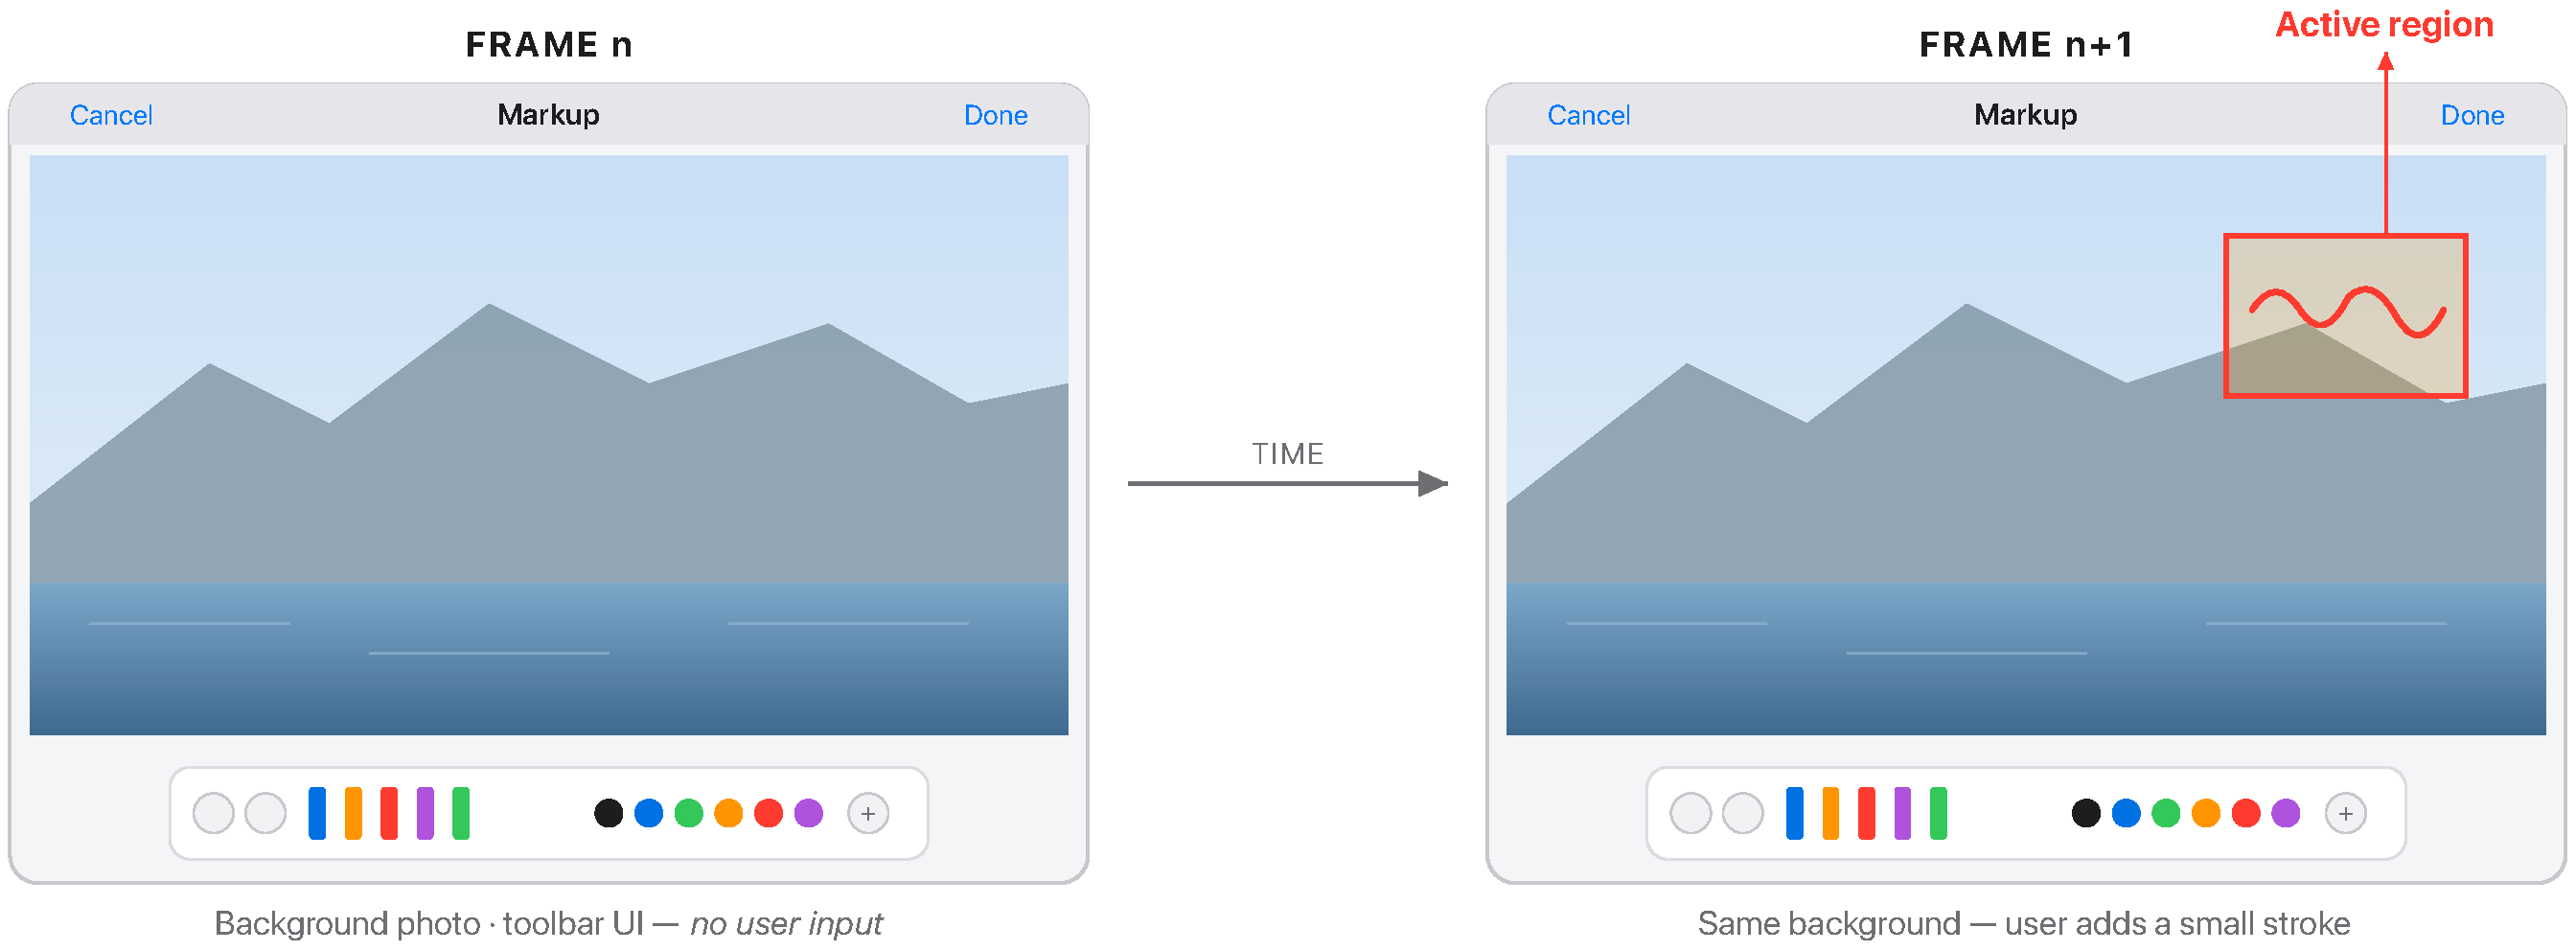
\includegraphics[width=0.64\textwidth]{figures/bru_motiv.pdf}
  \caption{Motivation for BRU. In sparse-activity content, only a small region
  changes between frames. A conventional decoder still reads the reference
  frame and writes a complete new frame for every decoded frame.}
  \label{fig:bru_motiv}
\end{figure*}

\subsection{Superblock Modes and Signaling}
Each superblock of a BRU frame is labeled \emph{active}, \emph{support}, or
\emph{inactive} (\code{bru\_mode}). Active superblocks are coded normally.
Inactive superblocks are copies of the collocated superblocks of the BRU
reference frame. Support superblocks form a one-superblock ring around each
active region; they are also copies, but the decoder reconstructs them so that
intra prediction and in-loop filtering at the edge of the active region see
correct neighboring samples. Because of the support ring, no coding tool needs
special rules at the boundary of an active region.

Inactive and support superblocks are not parsed. They use an implied inter
mode (Table~\ref{tab:bru_mode}): the whole superblock is one inter block that
uses the BRU reference with a zero MV and no residual.

\begin{table}[t]
\centering
\caption{Implied coding parameters of inactive and support superblocks in BRU.}
\label{tab:bru_mode}
\renewcommand{\arraystretch}{1.15}
\begin{tabular}{@{}ll@{}}
\toprule
\textbf{Parameter} & \textbf{Value} \\
\midrule
Partition       & superblock size (implied split at frame boundary) \\
Prediction      & inter, skip mode off \\
Inter mode      & \code{NEWMV} \\
Reference       & BRU reference (\code{bru\_ref\_idx}) \\
MV              & $(0,0)$ \\
Residual        & none (\code{skip\_txfm} $=1$) \\
\bottomrule
\end{tabular}
\end{table}

The signaling is hierarchical, so that the common cases are cheap. A
sequence-level flag enables BRU. In the frame header, \code{use\_bru} turns
BRU on for the frame and \code{bru\_ref\_idx} selects the BRU reference
frame. If the whole frame is unchanged, \code{bru\_inactive} marks all
superblocks inactive. Otherwise, \code{bru\_tile\_active} in each tile group
can mark a whole tile as inactive. Only in the remaining tiles is
\code{bru\_mode} sent per superblock, and only when it is not implied.

\subsection{Decoding}
Fig.~\ref{fig:bru_pipe} shows the decoding process of a BRU-optimized
decoder. Only active superblocks are parsed and reconstructed; support
superblocks are predicted from the BRU reference; inactive superblocks need no
work at all. In-loop filters are skipped for any filter unit that lies
entirely on support or inactive superblocks, since those pixels did not
change. Finally, the reconstructed active and support superblocks are written
back into the BRU reference frame, which then becomes the decoded frame.

\begin{figure*}[t]
  \centering
  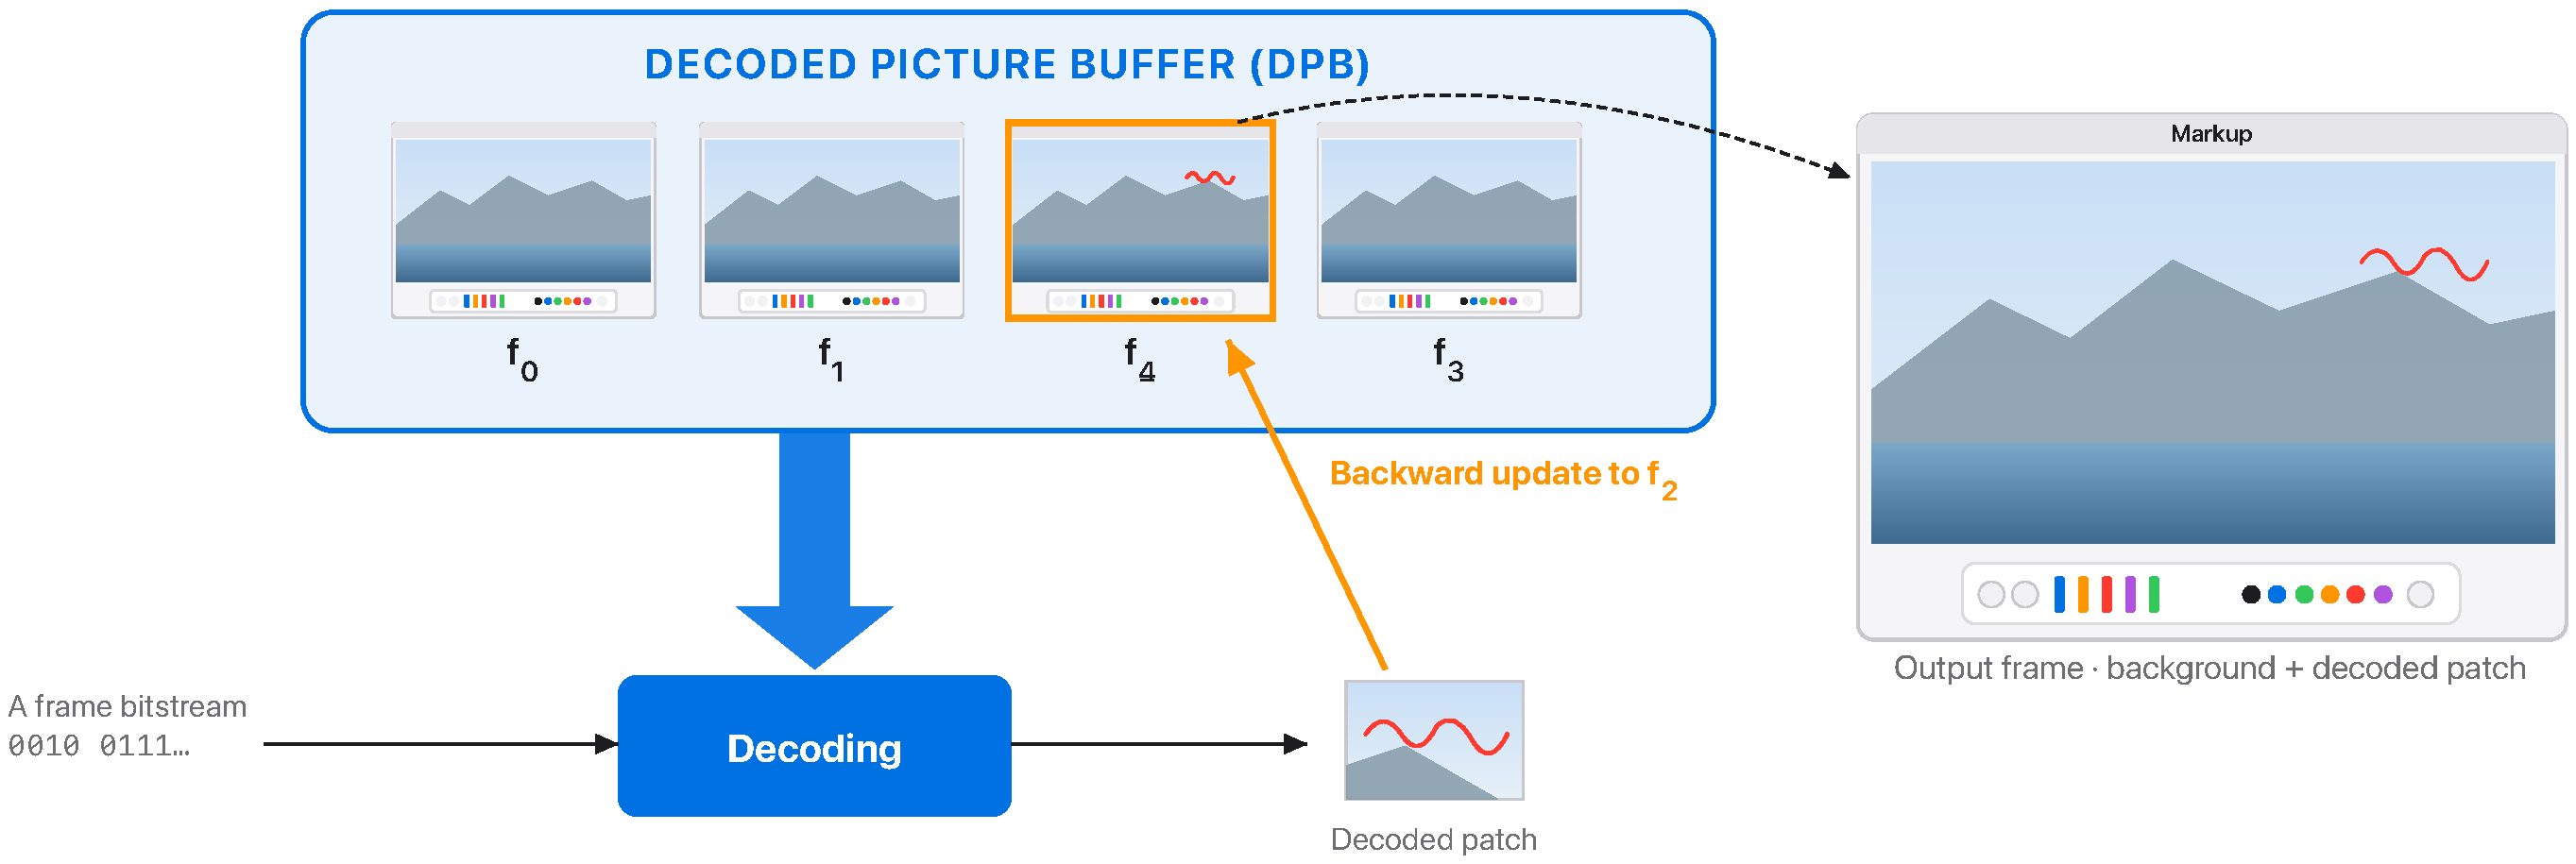
\includegraphics[width=0.74\textwidth]{figures/bru_pipe.pdf}
  \caption{BRU decoding. Only the active region of the frame is decoded. The
  decoded patch is written back into the BRU reference frame in the decoded
  picture buffer (DPB), which then serves as the output frame.}
  \label{fig:bru_pipe}
\end{figure*}

BRU is backward compatible with decoders that do not implement the in-place
update. Such a ``regular'' decoder decodes a BRU frame as a normal frame: it
copies inactive and support superblocks from the BRU reference into a new frame
buffer, and the normal reference refresh mechanism
(\code{refresh\_frame\_flags}) replaces the BRU reference with the new frame.
Both decoders produce identical output.

\subsection{Constraints}
Reading from and writing to the same picture buffer during decoding could
create read-after-write hazards. BRU prevents them with a few rules:
\begin{itemize}
  \item active superblocks may not use the BRU reference for inter
        prediction; only support and inactive superblocks read from it, and
        only at the collocated position;
  \item the motion field of the BRU reference is not used by motion field
        tools;
  \item Intra Block Copy may only reference active and support superblocks,
        which matters for $64{\times}64$ superblocks where the local search
        range could reach beyond the active region;
  \item each active region must be rectangular, active regions must not
        overlap, and the outermost superblocks of an active region must be
        support superblocks, except at the frame boundary.
\end{itemize}

%% =============================================================================
\section{Experimental Results}
\label{sec:results}
%% =============================================================================

\subsection{Test Conditions}
All tools were evaluated with the AV2 reference software, the AOMedia Video
Model (AVM) research-v13.0.0~\cite{avm_v13}, under the AOMedia
CTC~\cite{av2_ctc}. The test set contains seven classes: A1 (4K), A2
(1080p), A3 (720p), A4 (360p), A5 (270p), B1 (synthetic content such as
games), and B2 (screen content). Each sequence was coded at six quantization
indices, 110, 135, 160, 185, 210, and 235. The random access (RA) and low
delay (LD) configurations were tested; class A1 is not part of the LD tests.
Quality was measured by the peak signal-to-noise ratio (PSNR), averaged over
the Y, U, and V components with weights 14:1:1 (YUV-PSNR), and coding efficiency by the Bj{\o}ntegaard delta rate
(BD-rate)~\cite{BDrate-2001} computed with piecewise cubic interpolation.

Each test \emph{disables} one tool in the anchor, which has all tools enabled.
A positive $\Delta$BD-rate is therefore the extra bit rate needed without the
tool, i.e., the gain of the tool. Run times are given relative to the anchor;
a value below 100\% means the codec is faster without the tool, i.e., the tool
adds that much complexity. ``Overall'' is the average over classes A1--A5 and
B1. Screen content (B2) has very different statistics and is reported
separately.

Some improvements cannot be switched off in AVM because they replace an AV1
design rather than add a new tool: the reference frame system, the SMVP and
TMVP redesign, the DRL, the parametric wedge masks, and the MVD entropy
coder. Their contributions are part of the anchor and are not listed
separately.

\subsection{Per-Tool Results}

\begin{table*}[t]
\centering
\caption{BD-rate (\%, YUV-PSNR) and run time when individual tools are \emph{disabled}, random access (RA) configuration.
Positive values are the coding gain of the tool. Overall is the average over A1--A5 and B1.}
\label{tab:results_ra}
\renewcommand{\arraystretch}{1.12}
\begin{tabular}{@{}lrrrrrrrrrr@{}}
\toprule
\textbf{Tool} & \textbf{A1} & \textbf{A2} & \textbf{A3} & \textbf{A4} & \textbf{A5} & \textbf{B1} & \textbf{Overall} & \textbf{B2} & \textbf{EncT} & \textbf{DecT} \\
\midrule
TIP          & 1.48 & 1.41 & 1.72 & 2.03 & 1.97 & 0.46 & \textbf{1.40} & 0.30  & 105\% & 92\% \\
OPFL         & 0.62 & 0.89 & 0.81 & 0.98 & 0.99 & 0.71 & \textbf{0.82} & 0.24  & 93\%  & 89\% \\
AMVD         & 0.75 & 0.72 & 0.41 & 0.27 & 0.67 & 0.72 & \textbf{0.63} & 0.14  & 80\%  & 99\% \\
SMVR         & 0.85 & 0.59 & 0.55 & 0.28 & 0.28 & 0.50 & \textbf{0.55} & 0.06  & 97\%  & 99\% \\
BAWP         & 1.24 & 0.20 & 0.12 & 0.37 & $-0.01$ & 0.23 & \textbf{0.35} & 3.48 & 96\% & 100\% \\
RefMV bank   & 0.43 & 0.42 & 0.11 & 0.03 & 0.23 & 0.47 & \textbf{0.33} & 1.45  & 97\%  & 100\% \\
JMVD         & 0.40 & 0.27 & 0.14 & 0.08 & 0.28 & 0.24 & \textbf{0.24} & 0.23  & 97\%  & 101\% \\
IWM          & 0.26 & 0.21 & 0.14 & 0.23 & 0.18 & 0.08 & \textbf{0.18} & $-0.04$ & 100\% & 99\% \\
MV trajectory& 0.11 & 0.18 & 0.09 & 0.07 & 0.22 & 0.21 & \textbf{0.15} & 0.14  & 98\%  & 96\% \\
\bottomrule
\end{tabular}
\end{table*}

\begin{table}[t]
\centering
\caption{BD-rate (\%, YUV-PSNR) and run time when individual tools are \emph{disabled}, low delay (LD) configuration. OPFL, SMVR, and JMVD were not evaluated in LD.}
\label{tab:results_ld}
\renewcommand{\arraystretch}{1.12}
\setlength{\tabcolsep}{2.2pt}
\begin{tabular}{@{}lrrrrrrrrr@{}}
\toprule
\textbf{Tool} & \textbf{A2} & \textbf{A3} & \textbf{A4} & \textbf{A5} & \textbf{B1} & \textbf{Ovr.} & \textbf{B2} & \textbf{EncT} & \textbf{DecT} \\
\midrule
TIP        & 0.41 & 0.28 & 0.69 & 0.63 & $-0.01$ & \textbf{0.35} & $-0.02$ & 99\%  & 97\% \\
AMVD       & 0.74 & 0.41 & 0.41 & 0.51 & 0.82 & \textbf{0.64} & 0.36 & 100\% & 101\% \\
BAWP       & 0.36 & 0.13 & 0.37 & $-0.31$ & 0.33 & \textbf{0.26} & 3.27 & 95\% & 101\% \\
RefMV bank & 0.49 & $-0.05$ & 0.14 & 0.18 & 0.39 & \textbf{0.31} & 2.44 & 97\% & 99\% \\
MV traj.   & 0.23 & 0.06 & 0.36 & 0.03 & 0.28 & \textbf{0.21} & 0.26 & 98\% & 93\% \\
IWM        & 0.03 & $-0.04$ & 0.09 & $-0.11$ & $-0.03$ & \textbf{0.00} & $-0.11$ & 100\% & 100\% \\
\bottomrule
\end{tabular}
\end{table}

Tables~\ref{tab:results_ra} and~\ref{tab:results_ld} list the results for RA
and LD, respectively. We make the following observations.

\emph{TIP} gives the largest gain of any single tool in RA, 1.40\% overall and
about 2\% for the low-resolution classes A4 and A5. Disabling TIP makes the
encoder 5\% slower, most likely because the direct output mode and the cheap
TIP reference let the encoder skip part of its mode search; it makes the
decoder 8\% faster, which is the cost of producing the TIP prediction. In LD, TIP has to extrapolate from two
past references and its gain drops to 0.35\%.

\emph{Decoder-side refinement} is the second most important group. OPFL and
SMVR together give 1.37\% in RA. Both add decoder computation (11\% for OPFL
and 1\% for SMVR) and also encoder run time, since the encoder must run the
same refinement when it evaluates compound modes. They require references on
both sides of the current frame and so do not apply to LD.

\emph{MV coding tools} give consistent gains in both configurations: AMVD
gives 0.63\% in RA and 0.64\% in LD, and JMVD a further 0.24\% in RA. AMVD has
a large effect on encoder run time in RA (disabling it reduces the encoder
time to 80\%), which we attribute to the additional search over AMVD modes,
while it does not affect the decoder.

\emph{BAWP} gives a modest 0.35\% overall but 3.48\% (RA) and 3.27\% (LD) on
screen content, where fades and brightness changes are common. It also gives 1.24\% on class A1. The
\emph{reference MV bank} gives 0.33\% (RA) and 0.31\% (LD), and again much
more on screen content (1.45\% and 2.44\%), presumably because the same motion,
such as scrolling, repeats over large non-adjacent areas.

\emph{MV trajectory tracking} gives 0.15\% in RA and 0.21\% in LD. Its
decoder cost (4\% and 7\%) comes from the more complex motion field
construction. \emph{IWM} helps only blocks near picture boundaries and gives
0.18\% in RA at no measurable complexity.

\subsection{Warp Tools}

\begin{table*}[t]
\centering
\caption{BD-rate (\%, YUV-PSNR) and encoding time when warp tools are progressively disabled.
Test~1 (T1): warp causal disabled. Test~2 (T2): T1 plus warp extend disabled. Test~3 (T3): T2 plus warp delta disabled (all new warp modes off).}
\label{tab:results_warp}
\renewcommand{\arraystretch}{1.12}
\begin{tabular}{@{}lrrrrrrrrrrrr@{}}
\toprule
 & \multicolumn{6}{c}{\textbf{Random access}} & \multicolumn{6}{c}{\textbf{Low delay}} \\
\cmidrule(lr){2-7}\cmidrule(l){8-13}
 & \multicolumn{3}{c}{$\Delta$BD-rate} & \multicolumn{3}{c}{EncT} & \multicolumn{3}{c}{$\Delta$BD-rate} & \multicolumn{3}{c}{EncT} \\
\cmidrule(lr){2-4}\cmidrule(lr){5-7}\cmidrule(lr){8-10}\cmidrule(l){11-13}
\textbf{Class} & T1 & T2 & T3 & T1 & T2 & T3 & T1 & T2 & T3 & T1 & T2 & T3 \\
\midrule
A1 & 0.30 & 0.39 & 2.06 & 98\% & 96\% & 88\% & -- & -- & -- & -- & -- & -- \\
A2 & 0.37 & 0.50 & 3.54 & 98\% & 96\% & 87\% & 0.69 & 0.88 & 5.15 & 99\% & 94\% & 86\% \\
A3 & 0.33 & 0.56 & 4.69 & 99\% & 97\% & 92\% & 0.61 & 1.23 & 5.20 & 98\% & 91\% & 84\% \\
A4 & 0.24 & 0.52 & 8.59 & 104\% & 97\% & 97\% & 1.17 & 1.46 & 11.41 & 98\% & 91\% & 93\% \\
A5 & 0.21 & 0.34 & 4.37 & 102\% & 96\% & 96\% & 0.27 & 0.58 & 3.68 & 99\% & 96\% & 90\% \\
B1 & 0.36 & 0.47 & 3.92 & 97\% & 95\% & 86\% & 0.32 & 0.51 & 4.06 & 99\% & 95\% & 87\% \\
\midrule
\textbf{Overall} & \textbf{0.33} & \textbf{0.48} & \textbf{4.18} & 99\% & 96\% & 89\% & \textbf{0.62} & \textbf{0.91} & \textbf{5.60} & 98\% & 91\% & 87\% \\
B2 & 0.95 & 0.98 & 2.52 & 102\% & 97\% & 97\% & 0.92 & 2.72 & 4.12 & 98\% & 94\% & 96\% \\
\bottomrule
\end{tabular}
\end{table*}

The warp tools were evaluated by disabling them one after another
(Table~\ref{tab:results_warp}), so the gain of each tool is the difference
between consecutive tests. Compound warp causal gives 0.33\% (RA) and 0.62\%
(LD). Warp extend adds 0.15\% (RA) and 0.29\% (LD): reusing a neighbor's model
captures warped motion over a region at the cost of only an MV. Warp delta,
which includes the WRL, warp-mv, and warp-new-mv, gives by far the most:
3.70\% (RA) and 4.69\% (LD). Together, the AV2 warp tools save 4.18\% in RA and
5.60\% in LD, more than any other group of tools in this paper, and up to
11.41\% for class A4 in LD. Their gain is larger in LD; a likely reason is that
LD references are farther away in time, so zoom and rotation accumulate. The cost is mainly on
the encoder side, which becomes 11\% (RA) and 13\% (LD) faster when all warp
tools are disabled, mostly because of the parameter search in warp delta. The
decoding time is about the same in all tests.

\subsection{BRU}
BRU targets a specific use case, so it was evaluated separately, on
sparse-activity content in the LD configuration with three references. With
BRU, the encoding and decoding run times drop to 59\% and 51\% of the anchor,
respectively, i.e., by about 41\% and 49\%, at a cost of 3.40\% in BD-rate.
The coding loss is the price of the constraints in Section~\ref{sec:bru}; for
the target applications, the large savings in power, memory traffic, and
latency are far more important. Note that the run-time savings above are
measured in software; in a hardware decoder, the reduction of memory traffic,
which scales with the inactive area, is the main benefit.

%% =============================================================================
\section{Conclusion}
\label{sec:conclusion}
%% =============================================================================

This paper presented the inter coding tools of AV2. Compared with AV1, AV2
redesigns the reference frame system; adds temporal interpolated prediction,
decoder-side MV refinement, a much richer set of warp modes, parametric and
implicit wedge masks, and weighted prediction; improves MV prediction with a
simplified spatial search, trajectory-based and compressed temporal MV
prediction, and a reference MV bank; and improves MV coding with a larger
range, flexible precision, adaptive and joint MVDs, and shell-based MVD
coding. For low-power applications, BRU lets a decoder update only the changed
parts of a frame. Throughout, the design favors tools that let the decoder
derive information rather than receive it, and keeps memory bandwidth and
on-chip storage bounded for hardware decoders. The experiments show that the
individual tools give gains from a few tenths of a percent up to several
percent, and that together they are an important part of the roughly 30\%
coding efficiency improvement of AV2 over AV1.

\section*{Acknowledgment}
The authors thank all AOMedia members who contributed to the development of
the AV2 inter coding tools and to the AVM reference software.

\bibliographystyle{IEEEtran}
\bibliography{refs}

\end{document}
